% !TeX spellcheck = si_SI
% Predloga za pisanje zaključnih nalog
\documentclass[12pt,a4paper,twoside,fleqn,openright]{book}

% use quite a lot of packages
\usepackage[a-3u]{pdfx}
\usepackage{pdfpages}
\usepackage{amsfonts,amssymb,amsmath}
\usepackage[fleqn]{mathtools}
\usepackage{physics} 
\usepackage{esvect}
\usepackage{enumerate}
\usepackage[section]{placeins}
\usepackage[makeroom]{cancel}
\usepackage{float}
\usepackage[slovene]{babel}
\usepackage[utf8]{inputenc}
\usepackage{graphicx}
\usepackage{tikz}
\usepackage{ifthen}
\usepackage{fancyhdr}
\usepackage{epstopdf}
\usepackage{enumitem}
\usepackage{notoccite}
\usepackage{longtable}
\usepackage{hyperref}
\usepackage{ifoddpage}
\usepackage{tocloft}
\usepackage{titlesec}
\usepackage{pdfpages}
\usepackage{nameref}
\usepackage{multirow}
\usepackage{caption}
\usepackage{subcaption}
\usepackage{url}
\usepackage{icomma}
\usepackage{hyperref}
\usepackage{cite}
\usepackage[numbib]{tocbibind}
\usepackage[slovene]{datetime2}
\usepackage[inner=30mm,
            outer=25mm,
            top=30mm,
            bottom=25mm]{geometry}





% paragraph settings
\setlength\parindent{0pt}
\setlength{\parskip}{1.5ex plus 0.5ex minus 0.5ex}

% Hyphenating settings
\spaceskip=1.2\fontdimen2\font plus 1.3\fontdimen3\font minus 1.3\fontdimen4\font

% set equation environment indentation
\setlength{\mathindent}{0.5cm}%

% set itemize environment whitespacing and left margin
\setlist[itemize]{noitemsep,nolistsep, leftmargin=*}

% set table and figure captions
\captionsetup[table]{skip=10pt,singlelinecheck=false}
\captionsetup[figure]{justification=centering}

% set tablename to Preglednica
\AtBeginDocument{%
  \renewcommand\tablename{Preglednica}
}

% command for multiline cell in table
\newcommand{\minitab}[2][l]{\begin{tabular}{#1}#2\end{tabular}}

% opens a new page if current page is even
\newcommand{\addifeven}{
\checkoddpage
\ifoddpage
\else
\mbox{}
\newpage
\fi}

% set section and tableofcontents depth
\setcounter{secnumdepth}{3}
\setcounter{tocdepth}{3}
\def\labelitemi{--}

%  accordingly format a chapter definition
\titleformat{\chapter}[display]
  {\bfseries}{}{0pt}{\Huge\thechapter\quad}

% set fancy_nohead fancy header
\fancypagestyle{fancy_nohead}{
\fancyhead{}
\fancyfoot[LE,RO]{\thepage}
\renewcommand{\headrulewidth}{0pt}
\chead{}
\cfoot{}
}


% assign no_header
\assignpagestyle{\chapter}{fancy_nohead}

% table, fig and eq formatting

\renewcommand{\thetable}{\arabic{chapter}.\arabic{table}}
\renewcommand{\thefigure}{\arabic{chapter}.\arabic{figure}}
\renewcommand{\theequation}{\arabic{chapter}.\arabic{equation}}

\renewcommand\cftchapdotsep{\cftdotsep}  % adds leader dots from chapter titles to page numbers

% month year date format
%\DTMlangsetup{showdayofmonth=false}


\begin{document}

    % Prve strani
    \pagenumbering{roman}
    % !TeX spellcheck = si_SI
%Urejanje platnic, naslovnice, UDK, povzetka in kazal
%

% NOTRANJA NASLOVNICA
% !TeX spellcheck = sl_SI
% Notranja naslovnica
\thispagestyle{empty}
\begin{center}
    \begin{figure}[!hb]
        \centering
        \includegraphics[width=0.25\textwidth]{0 prveStrani/UNI-logo in FS-color-SLO-curve.jpg}
    \end{figure}
    \mbox\par\par \vspace*{-0.50cm} Magistrski študijski program druge stopnje 
    \\ \textbf{ STROJNIŠTVO - Razvojno raziskovalni program}
    
    \Large \mbox\par\par \vspace*{1.0cm}\textbf{MAGISTERSKI PRAKTIKUM}
    \\ \Large \mbox\par\par \vspace*{-0.75cm}\textbf{Poročilo}
    \\ \vspace{3cm} \normalsize
\end{center}

\normalsize{
    \textbf{Študent:} Gašper Bizjan \hfill \textbf{Vpisna št:} 23202100 \vspace{1cm}\\
    \textbf{Naslov teme Magisterskega praktikuma:}\\ Dinamika 3D natisnjenih termoaktivnih metamaterialnih blažilcev \vspace{1.5cm} \\
    \textbf{Naziv laboratorija:}\\ LADISK - Laboratorij za dinamiko strojev in konstrukcij \vspace{0.2cm}\\
    \textbf{Mentor v laboratoriju FS:} prof. dr. Janko Slavič, univ. dipl. inž.\\
    \vspace{2cm}\\
    \textbf{Kraj in datum:} Ljubljana, \today
    \vfill
    Podpis študenta: ..................... \hfill Podpis mentorja v laboratoriju: ......................
}


\setcounter{page}{1} 
\newpage
\mbox{}\thispagestyle{empty}
\newpage
\hypersetup{pageanchor=true} % no page anchors for the empty-pagestyle pages


% KAZALA
\input{0 prveStrani/kazala} 
    \newpage
    % !TeX spellcheck = si_SI
\addifeven

\vspace*{0mm}
\Large\textbf{Seznam uporabljenih simbolov}\normalsize
\vskip\medskipamount
\leaders\vrule width \textwidth\vskip0.4pt
\vskip\bigskipamount

\addcontentsline{toc}{section}{Seznam uporabljenih simbolov}

\begin{longtable}[l]{@{}p{.15\textwidth}@{}p{.15\textwidth}@{}p{.7\textwidth}@{}}
\hline
Oznaka & Enota & Pomen\\
\hline
\endhead
\hline
\endfoot
\hline
\endlastfoot
    $A$     & $\text{m}^2$          & površina preseka\\
    $b$     & m                     & globina nosilca\\
    $c$     & $\text{N s}^2/\text{m}$, J/kg K & koeficient dušenja, specifična toplota \\
    $d$, $\Delta$ & m, / & (brezdimenzijska) dolžina pomika kosinusnega nosilca \\ 
    $e$     & / & Eulerjevo število $2,71828...$ \\
    $E$     & Pa, J                 & modul elastičnosti ali energija\\
    $f$     & /, Hz & brezdimenzijska sila ali lastna frekvenca \\
    $F$     & N                     & sila \\
    $h$     & m, W/mK               & višina kosinusnega loka, toplotna prestopnost \\
    $i$     & /                     & imaginarno število $\sqrt{-1}$ \\
    $I$     & $\text{m}^4$, A       & vztrajnostni moment prereza, električni tok\\
    $k$     & N/mm                  & (nelinearna) togost\\
    $K$     & N/mm                  & linearna togost ROC\\
    $l, L$  & m                     & dolžina\\
    $\mathcal{L}$ & / & Lagrangian \\
    $m$ & kg & masa (resonatorja)\\
    $M$ & N m,  kg & moment ali  masa ROC \\
    $N$  & / & brezdimenzijska aksialna sila \\
    $P$    & N, W & sila ali moč \\
    $q$, $Q$ & /, m & (brezd.) relativna pr. stopnja ali vozliščni pomiki MKE\\ 
    $R$     & m, /,  $\Omega$           & radij nosilca, brezdimenzijska  lateralna sila ali el. upornost\\
    $s$, $S$ & m, / & (brezdimenzijska) dolžina aksialnega nosilca \\
    $t$     & m, s                  & globina nosilca, čas \\
    $T$ & $^\text{o}$C, / & temperatura ali prenosna funkcija \\ 
    $u$, $U$ & /, J, m, V & (normalizirana) energija, pr. stopnja ali el. napetost \\
    $v$, $V$ & /, m, m$^3$ & (brezdimenzijska) pr. stopnja resonatorja, volumen \\
    $w$, $W$ & / & (brezdimenzijski) pomik (kosinusnega nosilca)\\
    $\overline{w}$, $\overline{W}$ & m, / & (normirana) prva deformacijska oblika kosinusnega nosilca\\
    $x$, $X$ & /, m & (brezdimenzijska) prostostna stopnja \\

    \hline
    $[\,A\,]$   & /& dinamska matrika sistema \\
    $[\,B\,]$   & / & matrika odvodov oblikovnih funkcij \\
    $[\,C\,]$       & N $\text{s}^2$/m & disipacijska matrika\\
    $[\,D\,]$   & / & materialna matrika \\
    $[\,I\,]$   & /& identiteta \\
    $[\,J\,]$   & /& Jakobijeva matrika \\
    $[K]$       & Pa $\text{m}^2$/m & togostna matrika\\
    $[M]$       & kg & masna matrika\\
    $[\,N\,]$   & / & aproksimacijske funkcije \\
    $[\,T\,]$   &/ & transformacijska matrika \\
    

    &&\\
    $\alpha$ & / & brezdimenzijska togost   \\
    $\beta$ & /  &  brezdimenzijska masa \\
    $\gamma$ & / & razmerje dolžin \\
    $\delta$ & / &  koeficient brezdimenzijske sile tretje potence \\
    $\delta F$  & N & virtualna sila \\
    $\delta M$  & N m & virtualni moment\\
    $\delta W$  & J  & virtualno delo \\
    $\epsilon$ & / & brezdimenzijski red amplitude gibanja \\
    $\varepsilon$ & / & specifična deformacija \\
    $\zeta$ & /  & razmernik dušenja  \\
    $\eta$ & / &  koeficient brezdimenzijske sile pete potence \\
    $\theta$ & rad & kot horizontalne vzmeti \\ 
    $\kappa$ & 1/rad  &  krožna frekvenca resonatorja \\
    $\varkappa$ & / & razmerje krožnih frekvenc  \\ 
    $\lambda$ & / & lastne vrednosti \\
    $\mu$ & / & razmerje togosti ali disperzijska krivulja \\
    $\nu$ &  & Poissonov količnik \\
    $\pi$     & / & konstanta $3,1416...$ \\
    $\rho$  & kg/$\text{m}^2$   & gostota\\
    $\varrho$ & $\Omega$ mm$^2$/m & specifična električna upornost \\
    $\sigma$ & Pa & napetost \\
    $\tau$ & / & brezdimenzijski čas \\
    $\phi$ & rad, F & prostostna stopnja kota \\ 
    $\overline{\phi}$ & F & površinske sile \\
    $\overline{\Phi}$ & F & volumske sile \\
    $\omega$ & 1/rad  & krožna frekvenca ROC-ja\\
    $\Omega$ & / &  razmerje frekvence z lastno frekvenco ROC \\
    
    


\end{longtable}


\newpage
\begin{longtable}[l]{@{}p{.15\textwidth}@{}p{.85\textwidth}@{}}
\hline
Indeksi & \\
\hline
\endfirsthead
\hline
\endhead
    0 & začetno stanje, lastna frekvenca \\
    I,1 & 1. polje 1. glavnega sistema\\
    II,1 & 2. polje 1. glavnega sistema\\
    I,2 & 1. polje 2. glavnega sistema\\
    II,2 & 2. polje 2. glavnega sistema\\
    A & točka A\\
    b & upogibno \\
    B & točka B\\
    c & koncentrirano \\
    d & disperzijsko \\
    f & aktuacijsko \\
    g & steklenje \\
    h & horizontalno \\
    k & kinetično, končno \\
    KNT & kvazi ničelna togost \\
    MNT & mehanizem negativne togosti \\
    n & negativna\\
    $n1$ & negativna togost prvega območja \\
    $n2$ & negativna togost drugega območja \\
    $n3$ & negativna togost tretjega območja \\
    N & notranje \\
    opt & optimalno \\
    p & pozitivno, potencialno, konstanten tlak\\
    ROC & reprezentativna osnovna celica \\
    s, S & tlačno, površinsko \\
    sd & standardna deviacija \\
    sp & spodnja \\
    sr & srednja \\
    t & celotno \\
    v & vertikalno, volumsko \\
    Z & zunanje \\
    zg & zgornja \\
    $\infty$ & neskončno oddaljeno \\

\end{longtable}

\newpage

\addifeven

\vspace*{0mm}
\Large\textbf{Seznam uporabljenih okrajšav}\normalsize
\vskip\medskipamount
\leaders\vrule width \textwidth\vskip0.4pt
\vskip\bigskipamount

\addcontentsline{toc}{section}{Seznam uporabljenih okrajšav}

\begin{longtable}[l]{@{}p{.2\textwidth}@{}p{.8\textwidth}@{}}
\hline
Okrajšava & Pomen\\
\hline
\endfirsthead
\hline
\endhead
&\\
    3D & tridimenzionalno \\
    DVB & dinamični vibracijski blažilec \\
    FPF & frekvenčna prenosna funkcija \\
    GPLA & polilaktična kislina z aditivom grafitnega prahu \\ 
         &(ang. \emph{Graphite Polylactic Acid})\\
    KE & končni element \\
    KNT & kvazi ničelna togost \\
    KS & koordinatni sistem \\
    MKE & metoda končnih elementov \\
    MM & metamateriali \\
    MNT & mehanizem negativne togosti \\
    NT & negativna togost \\
    PLA & polilaktična kislina (ang. \emph{Polylactic acid})\\
    PT & pozitivna togost \\
    PZF & pasovno zavrnitveni filter \\
    ROC & reprezentativna osnovna celica \\
    VSND & visoka statična in nizka dinamična \\
\end{longtable}

\newpage

    \newpage \mbox{}
    \addifeven
    \newpage
    
    %change header and foot for non-chapter pages
    \renewcommand{\chaptermark}[1]{\markboth{#1}{}}
    \fancyhf{}
    \fancyhead[RO]{\nouppercase{\leftmark}}
    \fancyhead[LE]{\nouppercase{\leftmark}}
    \fancyfoot[LE,RO]{\thepage}
    \renewcommand{\headrulewidth}{0.1mm}
    \renewcommand{\footrulewidth}{0mm}
    \cfoot{}
    \setlength{\headheight}{15pt}
    \pagestyle{fancy}
    \pagenumbering{arabic}
    
    % Jedro
    % !TeX spellcheck = si_SI
\chapter{Uvod}\label{cha:uvod}
\section{Ozadje problema}\label{sec:ozadje_problema}
    
    Prisotnost nenadzorovanih vibracij v inženirskih aplikacijah hitro vodi v prekomerno obrabo, poškodbe ali celo v kritično in nevarno odpoved materiala ter strojnih delov. Z implementacijo vibroizolacije lahko omogočimo zaščito opazovanega sistema pred zunanjim povzročiteljem dinamičnih sil. 
    
    V praksi je največkrat uporabljena linearna vibroizolacija, ki je učinkoviti le, če je njena lastna frekvenca precej nižja od frekvence vzbujanja. Za odpravo te pomanjkljivosti je bila zasnovana nelinearna vibroizolacija z visoko statično in nizko dinamično (VSND) togostjo, ki izolira vibracije v nizkofrekvenčnem območju. Pri tem visoka statična togost pomeni veliko nosilnost, medtem ko nizka dinamična togost pomeni povečano območje izolacije pri nizkih frekvencah. Skoraj ničelna dinamična togost v delovni točki, ki je značilna za nelinearno vibroizolacijo, se imenuje kvazi ničelna togost (KNT), nelinearni izolatorji z značilnostmi KNT pa se v nadaljevanju imenujejo kvazi ničelni togostni izolatorji ali KNT izolatorji.
    
    Metamateriali (MM) so v zadnjih dveh desetletjih deležni vse večjega raziskovalnega zanimanja, saj imajo zanimive optične, elektromagnetne, akustične in mehanske lastnosti. Znani tudi pod imenom metastrukture, izražajo posebne fizikalne lastnosti, ki jih v naravi ne najdemo. Gre za serijo ponavljajočih se in geometrijsko skrbno načrtovanih podstruktur. Podobni so celičnim strukturam, njihove posebne fizikalne lastnosti, ki jih v naravi ne najdemo, pa je mogoče preučevati iz osnovne reprezentativne celice (ROC). Vibroizolativni MM sestoji iz periodično razporejenih lokalnih resonatorjev, ki absorbirajo vibracijsko energijo v določenem frekvenčnem območju. 
    
    Zaradi prostorske razporeditve osnovne celice se je aditivna tehnologija izkazala kot odlični proces za izdelavo metastruktur. Geometrijsko kompleksne podstrukture lahko skoraj poljubno postavimo v prostoru in jih na makronivoju formuliramo v MM poljubne oblike.

    Rešitev s pasivno vibroizolacijo ima prednost enostavnosti rešitve, brez kompleksnih mehanizmov, ki bi potrebovali zunanje napajanje ali krmiljenje. Negativna posledica je nezmožnost prilagajanja na spremembe delovnih pogojev stroja ali okolice. Rešitev predstavlja semi-pasivna vibroizolacija, ki omogoča regulacijo in prilagajanje na spremembe. 


\section{Cilji praktikuma}\label{sec:cilji_naloge}

    Osrednja problematika naloge je raziskava dinamike 3D tiskanih termoaktivnih metamaterialnih KNT vibroizolatorjev za uporabo v nizkofrekvenčnem področju.
    
    V prvem delu naloge predstavimo MM in nato potrebne teoretične osnove za formulacijo reprezentativne osnovne celice (ROC) MM, ki izkazuje VSND togost ali kvazi ničelno togost (KNT). Bistveno vlogo za doseganje KNT lastnosti nelinearnih vibroizolatorjev igrajo elementi z negativno togostjo (NT) imajo ključno vlogo pri oblikovanju funkcije KNT, saj nevtralizirajo pozitivno togostjo (PT) struktur. Značilnost NT se lahko uresniči iz različnih struktur, kot so poševne vzmeti, upogibni nosilci, magnetne vzmeti in biološko navdihnjene strukture. Pri metamaterialih lahko NT lastnost dosežemo z vključitvijo bistabilne strukture, ki ob preskoku iz enega v drugo stabilno stanje nasprotuje PT strukture.
    
    Večje število zaporednih ROC tvori enodimenzionalni KNT MM. Za dinamično analizo MM vibroizolatorja je opisana teorija dvomasnega dušilca nihanj. Z obravnavo MM kot neskončne periodične strukture lahko analitično določimo frekvenčno pasovno vrzel, v kateri je odziv sistema manjši. 
    
    Analitični popisi realnih struktur imajo svoje omejitve, saj je natančen popis geometrije nemogoč. S tem razlogom bomo dinamiko problema rešili z metodo končnih elementov (MKE). 
    
    Opišemo tudi teorijo MM, ki je izdelan z uporabo aditivne tehnologije, pri čemer uporabimo filament iz polilaktične kisline (PLA - \textit{Polylactic acid}) z aditivom grafitnega prahu - torej GPLA (\textit{Graphite Polylactic acid}), kar omogoča prevajanje elektrike skozi MM. Z uporovnim segrevanjem materiala preko Joulovega toka bomo dosegli njegovo mehčanje in zmanjšanje togosti, ki je bistvena lastnost pri obravnavi nihanja. Tako dosežemo adaptivni metamaterial, ki ima v primerjavi z pasivnimi vibroizolatorji prilagodljivo in posledično širše uporabno frekvenčno območje. Na GPLA vzorcih izmerimo potrebne materialne lastnosti za konkretno določitev parametrov ROC.
        
    Zadnji korak, ki bo del magistrske naloge, je meritev odziva na dinamične motnje v okolici lastnih frekvenc in vpliv izdelane MM vibroizolacije. Tukaj bomo z spreminjanjem delovnih pogojev želeli zmanjšati učinkovitost metamateriala, ki pa se bo zaradi svoje adaptivnosti bil zmožen novim parametrom prilagoditi.



    % !TeX spellcheck = sl_SI
   
    \chapter{Osnove metamaterialov}\label{sec:osnove_metamaterialov}

    Metamateriali (MM) so umetno strukturirani kompoziti, ki so zgrajeni iz periodično razporejenih gradnikov, ki ne le da izboljšujejo lastnosti osnovnega materiala, temveč dajejo tudi različne funkcionalnosti, kot so negativni lomni količnik, negativna masna gostota, negativno Poissonovo razmerje, negativna dielektričnost, negativna permeabilnost, negativna stisljivost, negativni koeficienta toplotnega raztezka in tako dalje. Lastnosti metamaterialov so spremenjene tako, da presegajo lastnosti, ki jih najdemo v naravi. Tam najdemo celične strukture, kot so votlosti v pluti ali kosteh, vendar tam ne gre za periodične strukture, vendar le naključno razporejene nehomogenosti materiala. Pravi MM imajo periodično razporejene reprezentativne osnovne celice (ROC). Povzeto po \cite{Dalela2022} in \cite{Ji2021}. 
    
    Prvi MM so bili uvedeni na elektromagnetnem področju, pozneje pa je bil koncept metamaterialov razširjen tudi na optiko, akustiko in navsezadnje tudi na mehaniko trdnih teles kot vibroizolator z negativno togostjo. Klasifikacijo MM lahko vidimo na sliki  \ref{fig:klasifikacija metamaterialov}. 
    
    \begin{figure}[!hb]
            \centering
            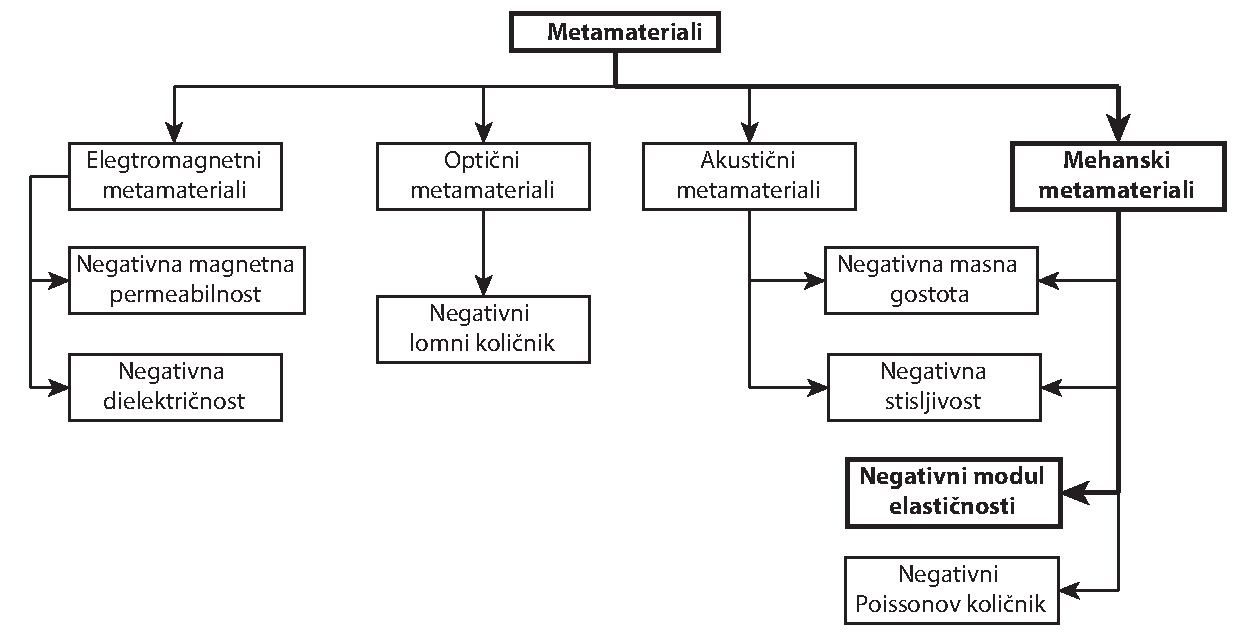
\includegraphics[width=\linewidth]{Magisterski praktikum/slike/teorija/klasifikacija_metamaterialov.pdf}
            \caption{Klasifikacija metamaterialov.}\label{fig:klasifikacija metamaterialov}
    \end{figure}

    \newpage
    
    Mehanski in akustični metamateriali med drugim vključujejo celične metamateriale, pomožne metamateriale z negativnim Poissonovim količnikom, pentamode metamateriale z znatno večjim stisljivostnim modulom kot strižnim modulom, metamaterialne strukture na osnovi origamija in materiale z lastnostjo pasovne vrzeli. Te vsi so obetavni za nadzor vibracij in zvoka. V našem primeru uporabimo koncept metamateriala z lastnostjo pasovne vrzeli. 
    
    Mehanske metamateriale za vibroizolacijo lahko razvijemo tako, da v glavni strukturi naredimo nekaj mehanskih podenot ali reprezentativnih osnovnih celic (ROC), tako da lahko mehanski valovi, ki se prenašajo v gradnikih, resonirajo s podenotami strukture. MM tako izraža lastnosti pasovno zavrnitvenega filtra (PZF), kar pomeni, da v določenem frekvenčnem območju MM ne dopušča, ali vsaj bistveno zmanjša širjenje valovanja. Naš cilj je torej razviti nov model MM za izboljšanje položaja in pasovne širine zavrnitvenega pasu. Obstajata dva pristopa za preučevanje značilnosti zapornih pasov: Braggovo sipanje (\textit{ang. Bragg scattering}) in princip lokalnih resonanc. 
    
    Kadar je širjenje valovanja odvisno le od periodične razporeditve in velikosti ROC v mediju, se te imenujejo fononski kristali. Pri fononskih kristalih je ena od najpomembnejših značilnosti učinek Braggovega sipanja, ki jih povzroči destruktivna interferenca prihajajočih in odbitih valov. Učinek Braggovega sipanja je omejen z velikostjo konstante mreže podstruktur. Na splošno so mere ROC v MM običajno manjše od valovne dolžine lastnosti, na katero vplivajo. Za dušenje visokih frekvenc posledično potrebujemo majhne, za nizkofrekvenčne PZF pa bi potrebovali zelo velike ROC, kar je iz vidika izdelave metamateriala nepraktično. 
    
    Rešitev omejitve velikosti je učinek lokalne resonance. Ta povzroči nizkofrekvenčno pasovno vrzel z mrežno konstanto, ki je za več redov manjša od valovne dolžine razširjajočih se valov. Fenomen pasovne vrzeli in pasovne širine, ki nastane zaradi lokalne resonance, je odvisen od geometrijskih parametrov in materialnih lastnosti resonatorjev; ni odvisen od periodičnosti in razporeditve ROC. Običajno to pomeni, da je vsaka ROC sistem masa-vzmet, katere lastna frekvenca $\omega_0=\sqrt{k/m}$ je odvisna od togosti $k$ njene interne vzmeti in mase $m$ (poglavje \ref{sec:dvomasni_dušilec_nihanj}). Za nizkofrekvenčno izolacijo vibracij mora biti bodisi masa zelo velika bodisi togost majhna. Resonator je omejen z veliko maso ali majhno togostjo. Da bi premagali to omejitev lahko v ROC z obstoječo pozitivno togostjo (PT) dodamo negativno togost (NT) in tako linearno togost spremenimo v nelinearno. Tako dosežemo kvazi ničelno togost (KNT), kar omogoča PZF zelo nizkih frekvenc.  
    
    V sledečem poglavju \ref{sec:ROC_statika} matematično zasnujemo ROC z KNT preko enačb strukturne statike in stabilnosti.
    
    
\newpage
\chapter{Analitična izpeljava ROC}\label{sec:ROC_statika}

    V sledečem poglavju zasnujemo reprezentativno osnovno celico (ROC) z visoko statično in nizko dinamično togostjo (VSND), ki ima lastnost kvazi ničelne togosti (KNT) (\cite{dalela2022design, fan2020design, cai2020design} ). Za primer sistema z eno prostostno stopnjo, sposobnost pasivnega dušenja pri nizkih frekvencah zavisi od sposobnosti zagotoviti majhno togost ali veliko maso sistema. Ker je masa najpogosteje nespremenljiva, želimo čim manjšo togost, kar pa pomeni nesposobnost prenašanja večjih statičnih obremenitev. Torej želimo vibroizolacijo, kjer prvotno statično obremenitev prevzame visoka togost, dinamične obremenitve pa se srečajo z nizko togostjo. VSND togost dosežemo z nelinearno vzmetjo s KNT, ki jo dobimo tako, da pozitivni togosti nasprotujemo z negativno togostjo. Najbolj tipični KNT vibroizolator \cite{lan2014design} je sestavljen iz treh vzmeti - iz vertikalne vzmeti, ki nosi statične obremenitve na tlak in zagotavlja pozitivno togost $k_p$ ter dveh paralelno vezanih horizontalnih vzmeti. Te nudijo negativno togost $k_n$, ki izniči pozitivno togost navpične vzmeti (slika \ref{fig:vzmetna_KNT_ROC}). Za našo aplikacijo metamateriala narejenega z aditivno tehnologijo, kjer je ROC zvezna struktura, moramo vzmeti nadomestiti s strukturam prijazni metodi izdelave. Pozitivno togost lahko tvorimo z navpičnimi ukrivljenimi nosilci in negativno togost z ukrivljenimi horizontalnimi nosilci, kjer imamo ob obremenitvi preskok sistema. Nosilci so zaprti znotraj bolj togega okvirja (slika \ref{fig:3D tiskana_KNT_ROC}).
    \begin{figure}[!htb]
        \centering
        \begin{subfigure}{.4\textwidth}
            \centering
            \includegraphics[trim=0 0 -2cm 0, clip, width=\linewidth]{Magisterski praktikum/slike/teorija/vzmetna_KNT_ROC.png}
            \caption{}
            \label{fig:vzmetna_KNT_ROC}
        \end{subfigure}%
        \begin{subfigure}{.3\textwidth}
            \centering
            \includegraphics[trim=-5cm 0 0 0, clip, width=\linewidth]{Magisterski praktikum/slike/teorija/3D tiskana_KNT_ROC.png}
            \caption{}
            \label{fig:3D tiskana_KNT_ROC}
        \end{subfigure}%
        \caption{(a) Vzmetni KNT mehanizem in (b) 3D tiskana KNT ROC.}
    \end{figure}
    
    V sledečem poglavju analitično z enačbami, statike, trdnosti in stabilnosti zasnujemo KNT ROC. Sprva izpeljemo enačbe za navpične nosilce za pozitivno togost $k_p$ in nato enačbe za poševne nosilce z negativno togostjo $k_n$. Z glavnim pogojem KNT  povežemo vse nosilce skupaj v ROC z KNT: 
    \begin{align}\label{eq:pogoh_KNT}
        \frac{1}{2} (2 k_p +  k_n) = 0 \,.
    \end{align}
    
    
    \newpage
    \section{Izpeljava elementa s pozitivno togostjo}\label{sec:Izpeljava_elementa_s_pozitivno_togostjo}
    
        Pozitivni element je sestavljen iz simetričnih ukrivljenih nosilcev z togostjo $k_p$ in ga obravnavamo kot en sam Eulerjev-Bernoullijev nosilec, pri čemer upoštevamo le notranji moment (slika \ref{fig:diagram prostega telesa pozitivni element}). Zaradi simetrij obravnavamo le polovico enega od nosilcev in ga predstavimo v diagramu prostega telesa.
        \begin{figure}[!hb]
                \centering
                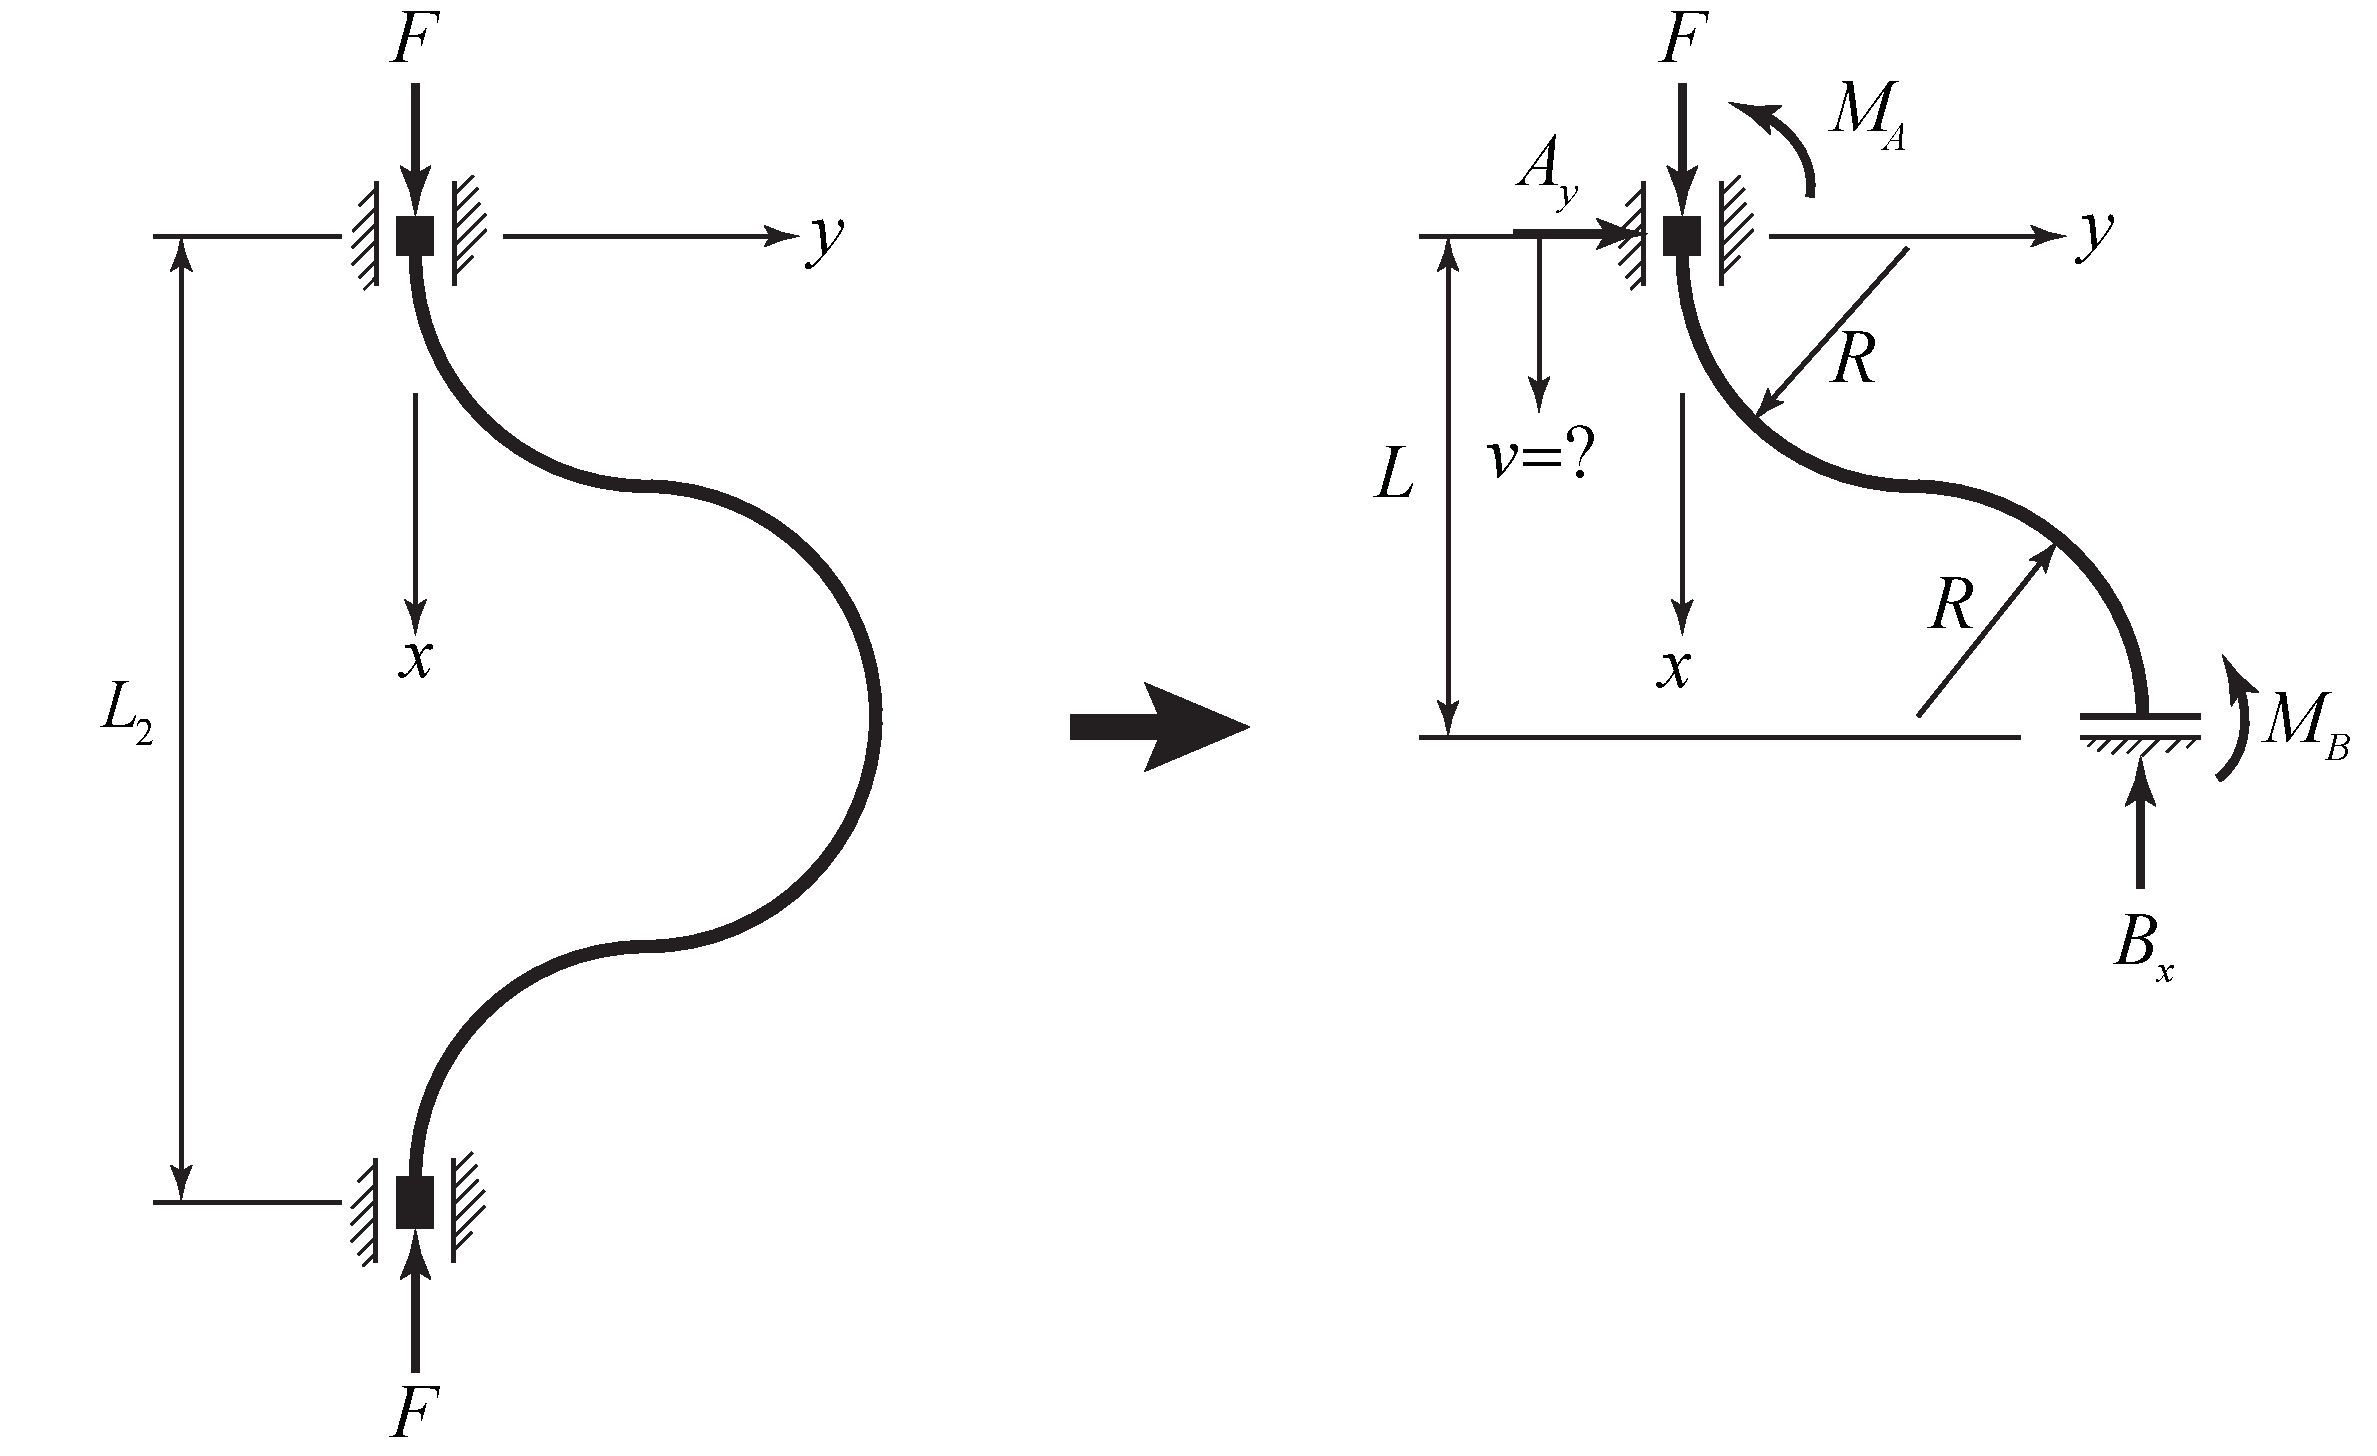
\includegraphics[scale=0.32]{Magisterski praktikum/slike/teorija/pozitivni_nosilec_poenostavitev.pdf}
                \caption{Diagram prostega telesa problema.}\label{fig:diagram prostega telesa pozitivni element}
        \end{figure}
        
        Osnovni sistem je statično nedoločen in ga razdelimo na dva določena glavna sistema, kjer je prvemu sistemu odvzeta momenta reakcija, ki se pojavi v drugem sistemu kot obremenitev (slika \ref{fig:glavni in virtualni sistemi}).
        \begin{figure}[!hb]
                \centering
                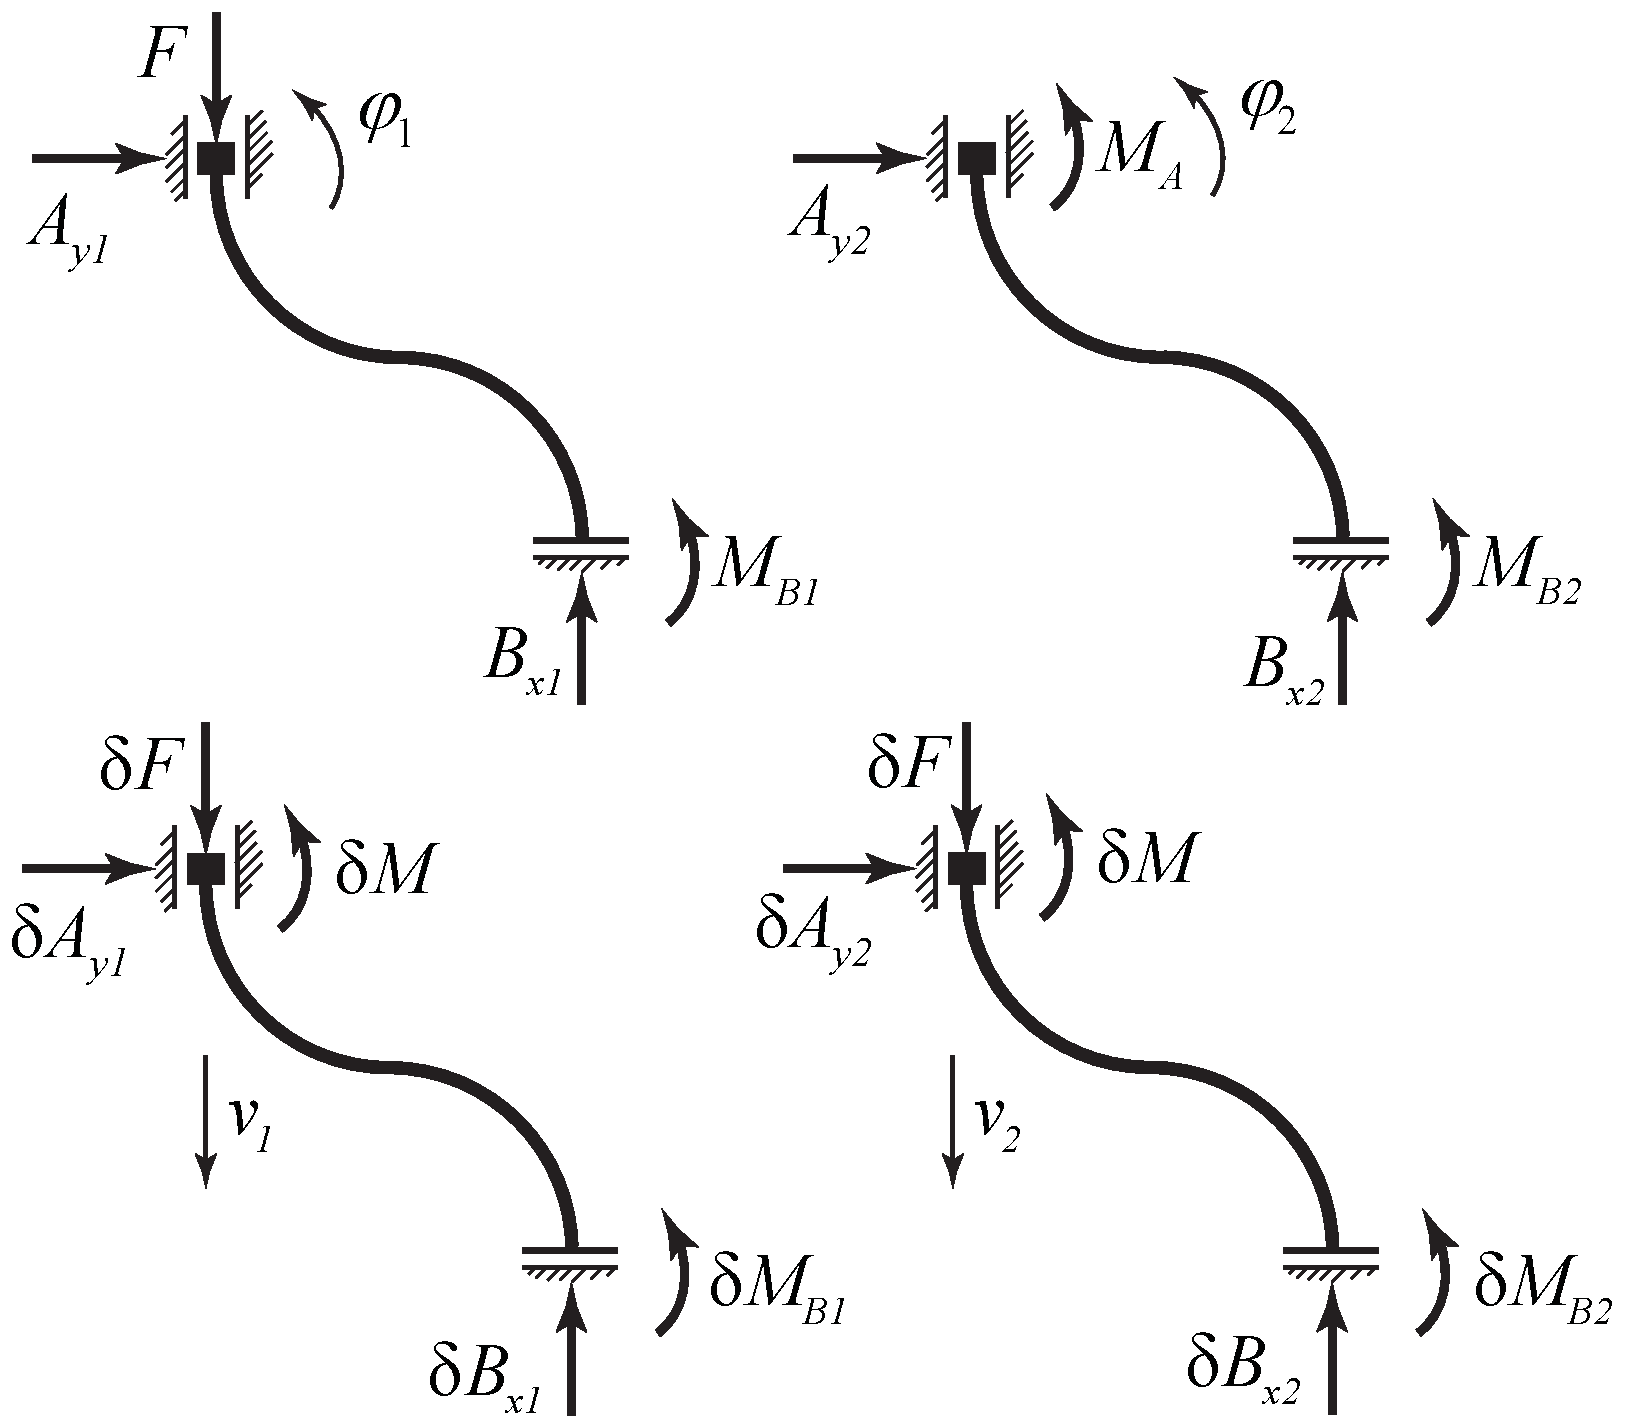
\includegraphics[scale=0.32]{Magisterski praktikum/slike/teorija/pozitivni_nosilec_sistemi.pdf}
                \caption{Glavni in virtualni sistemi.}\label{fig:glavni in virtualni sistemi}
        \end{figure}
    
    
        \newpage
        Za izračun pomika togosti $k_p$ uporabimo virtualno delo, ki je aplikacija principa najmanjše akcije - virtualno delo, ki ga opravi virtualna obremenitev, bo vedno minimalen. Vsakemu od glavnih sistemov (ločeno) pripišemo virtualne obremenitve $\delta F$ in $\delta M$. Glavna sistema imata dve polji I in II, ki jih modeliramo kot četrtino krožnice  $\varphi \in [0, \varphi/2]$. Glavni sistem 1 z obremenitvijo $F$ in glavni sistem 2 z obremenitvijo $M_\text{A}$ imata notranje momente definirane kot:
        \begin{align}
            M_{\text{I},1}(\varphi) &= -FR (1-\cos\varphi) \nonumber \\ 
            M_{\text{II},1}(\varphi) &= -FR (1+\sin\varphi) \nonumber \\ 
            M_{\text{I},2}(\varphi) &= -M_\text{A} \nonumber \\ 
            M_{\text{II},2}(\varphi) &= -M_\text{A} \,,
        \end{align}
        kjer je $R$ polmer loka nosilca.  
        
        Virtualni moment $\delta M$ povzroča rotacijo v točki A in je uporabljen za izračun neznane reakcijske sile $M_A$. Notranje obremenitve virtualnih sistemov so: 
        \begin{align}
            \delta M_{\text{I},1} = \delta M_{\text{II},1} = \delta M_{\text{I},2}= \delta M_{\text{II},2} = - \delta M \,.
        \end{align}
        
        Virtualno delo notranjih obremenitev $\delta W_\text{N}$ in zunanjih obremenitev $\delta W_\text{Z}$, zaradi $N$ sil in $K$ momentov, je po principu virtualnih sil in momentov definirano kot:
        \begin{align}
            \delta W_\text{N} &=  \int_{s}^{} \frac{M  \, \delta M}{E I} \,\text{d}s =  \int_{\varphi}^{} \frac{M  \, \delta M}{E I} R \,\text{d}\varphi \, ,\\
            \delta W_\text{Z} &=  \sum_{i=1}^{N} \delta F_i \delta v_i + \sum_{j=1}^{K} \delta M_j \delta \varphi_j    \,,
        \end{align}
        pri čemer je $E$ modul elastičnosti in $I=I_1=b \, t_1^3 /12$ vztrajnostni moment prereza. \\ $b$ je globina in $t_1$ širina nosilca. Velja: 
        \begin{align}\label{eq:virtualno delo_enakost}
             \delta W_\text{N} = \delta W_\text{Z}\,.
        \end{align}
        
        Za prvi sistem lahko izračunamo in  nato iz enakosti v enačbi \eqref{eq:virtualno delo_enakost} dobimo $\varphi_1$:
        \begin{align}
             W_{\text{N}, 1} &= \int_{0}^{\pi/2} \frac{M_{\text{I},1} \, \delta M_{\text{I},1}}{E I} R \,\text{d}s +
             \int_{0}^{\pi/2} \frac{M_{\text{II},1}  \, \delta M_{\text{II},1}}{E I} R \,\text{d}\varphi =
             \pi  \, \frac{F R^2  \, \delta M}{E I} \,, \\
             W_{\text{Z}, 1} &= \delta M \, \varphi_1 \,,  \\
             \varphi_1 &= \pi \frac{F R^2}{E I} \,.
        \end{align}
        Podobno uporabimo notranje reakcije drugega glavnega in virtualnega sistema za:
        \begin{align}
             \varphi_2 &= \pi \frac{M_A}{E I} \,.
        \end{align}

        Dejanska rotacija je zaradi toge podpore omejena in velja pogoj $\varphi_1 + \varphi_2 = 0$, kar pomeni, da je momentna reakcija v podpori enaka:
        \begin{align}
             M_\text{A}= - F R \,.
        \end{align}
        
        \newpage
        Ker nas zanima togost $k_p=\Delta F / \Delta v$, potrebujemo skrček nosilca v navpični smeri $v$, ki je posledica delovanja virtualne sile $\delta F$ v točki A. Notranje obremenitve so:
        \begin{align}
            \delta M_{\text{I},1}(\varphi) &= \delta M_{\text{I},2}(\varphi) = -\delta F (1 - \cos\varphi) \nonumber \,,\\
            \delta M_{\text{II},1}(\varphi) &= \delta M_{\text{II},2}(\varphi) = -\delta F (1 + \sin\varphi) \,.
        \end{align}
        
        Podobno kot smo že prej, uporabimo notranje reakcije prvega in drugega glavnega ter virtualnega sistema in nato preko virtualnega dela dobimo:
        \begin{align}
            v_1 &= \frac{3 \pi}{2} \frac{F R^3}{E I} \, \text{ in} \\
            v_2 &= \pi \frac{M_A \, R^2}{E I} = - \pi \frac{F R^3}{E I}  \,.
        \end{align}
        
        Navpični pomik elementa s pozitivno togostjo $v_p$ povzroči dejanska sila $F$. Upoštevamo simetrijo, superpozicijo in dolžino celotnega nosilca, ki je $l_1=4 R$. Vidimo, da je:
        \begin{align}
            v_p = 2 ( v_1 + v_2 ) = \frac{\pi}{2^6} \frac{F l_1^3}{E I_1}  \,.
        \end{align}
        
        končno togost pozitivnega elementa izračunamo kot:
        \begin{align}\label{eq:kp}
            k_p = \frac{\Delta F}{\Delta v_p} = \frac{F-0}{v_p-0} = \frac{2^6}{\pi} \frac{E I_1}{l_1^3} \approx 20,372 \, \frac{E I_1}{l_1^3}\,.
        \end{align}
        
    \section{Izpeljava elementa z negativni togostjo}\label{sec:Izpeljava_elementa_z_negativno_togostjo}
    
        Element z negativno togostjo ROC sestoji iz štirih togo vpetih kosinusnih lokov dolžine $l_2$, globine $b$, debeline $t_2$, razdaljo od poravnane lege do srednje linije loka $h$ in modul elastičnosti $E$. Izpeljimo nadomestno togost iz sledeče bistabilnostne analize \cite{liu2000microelectromech} spodnjega elementa (slika \ref{fig:kosinusni nosilec}).
        \begin{figure}[!hb]
                \centering
                \includegraphics[trim=0 0 0.1cm 0.1cm, clip, scale=0.4]{Magisterski praktikum/slike/teorija/kosinusni nosilec.png}
                \caption{Shema kosinusnega nosilca.}\label{fig:kosinusni nosilec}
        \end{figure}
        
        \newpage
        Izhajamo iz enačbe Euler-Bernulijevega nosilca obremenjenega z aksialno silo $P$: 
        \begin{equation}
            E I_2 \frac{\dd ^4 w}{\dd x^4}+P \frac{\dd^2 w}{\dd x^2}=0 \, ,
        \end{equation}
        
        kjer je $w=w(x)$ prečni pomik nosilca. Togo vpet nosilec ima robne pogoje:
        \begin{equation}
            w(0)=w(l_2)=0, \quad\left(\frac{\dd w}{\dd x}\right)_{x=0}=\left(\frac{\dd w}{\dd x}\right)_{x=l_2}=0 \, .
        \end{equation}
        Vpeljemo definicijo normirane aksialne sile, ki je enaka:
        \begin{equation}
            N^2=\frac{P \, l_2^2}{E I_2} \, .
        \end{equation}
        
        Reševanje diferencialne enačbe vodi v pogojno enačbo:
        \begin{equation}
            \sin \left(\frac{N}{2}\right)\left[\tan \left(\frac{N}{2}\right)-\frac{N}{2}\right]=0 \,
        \end{equation}
        in dve vrsti rešitev, kjer je prva:
        \begin{equation}\label{eq:def_ob_1}
            \left.\begin{array}{l}
            w_j(x)=C\left[1-\cos \left(N_j \frac{x}{l_2}\right)\right] \\
            N_j=(j+1) \pi
            \end{array}\right\} \quad j = 1, 3, 5 \ldots
        \end{equation}
        in druga: 
        \begin{equation}\label{eq:def_obl_2}
            \begin{aligned}
            &\left.w_j(x)=C\left[1-2 \frac{x}{l_2}-\cos \left(N_j \frac{x}{l_2}\right)+\frac{2 \sin \left(N_j \frac{x}{l_2}\right)}{N_j}\right]\right\} \quad j=2, 4, 6 \ldots \\
            &N_j=2,86 \pi; \, 4,92 \pi \ldots
            \end{aligned}
        \end{equation}
        
        Zgornja analiza podaja matematično osnovo stabilnostne analize uklona nosilca. Namesto prednapetega nosilca, lahko izhajamo iz nosilca, katerega izhodišče je hkrati prva deformacijska oblika z enačbo:
        \begin{equation}
            \bar w(x)=\frac{h}{2}\left[1-\cos \left(2 \pi \frac{x}{l_2}\right)\right] \,.
        \end{equation}
        
        Ob obremenitvi nosilca z lateralno silo $F$ pri $x=l_2/2$, se središče nosilca ob predpostavki majhnih pomikov poda za $d$ in dolžina nosilca postane $s$: 
        \begin{align}\label{eq:dolzina_d}
            d &= \bar w \left(\frac{l_2}{2}\right)-w\left(\frac{l_2}{2}\right) \,, \\
            s &= \int_0^{l_2} \sqrt{1+\left(\frac{\dd w}{\dd x}\right)^2} \dd x \approx \int_0^{l_2}\left[1+\frac{1}{2}\left(\frac{\dd w}{\dd x}\right)^2\right] \dd x \,.
        \end{align}
        
        Sprememba $s$ povzroči nastanek aksialne sile: 
        \begin{equation}
            P = E \, b \, t \left(1 - \frac{s}{s_0}\right) \,,
        \end{equation}
        kjer je $s_0=l_2$ začetna dolžina nosilca. 
        
        Med deformacijo je prisotna upogibna energija $u_b$, tlačna energija $u_s$ in energija aktuacije $u_f$. Variacija energij je: 
        \begin{align}\label{eq:variacija_energij}
            \partial u_b &= \partial\left[\frac{E I}{2} \int_0^{l_2}\left(\frac{\dd^2 \bar{w}}{\dd x^2}-\frac{\dd^2 w}{\dd x^2}\right)^2 \dd x\right] \,,\\
            \partial u_s &= -P \partial s \,,\\
            \partial u_s &= -F \partial d \,.
        \end{align}
        
        Problem rešujemo s superpozicijo deformacijskih oblik. Deformacijske oblike po enačbah \eqref{eq:def_ob_1} in \eqref{eq:def_obl_2} so ortogonalne in jih lahko uporabimo tudi kot osnovo za izračun pomika $w$ prvotno deformiranega nosilca, saj so robni pogoji enaki. Sprva normiramo parameter:
        \begin{equation}
            X = \frac{x}{l_2} \,, \,\, W(X)=\frac{X l_2}{h}  \, .
        \end{equation}
        
        Torej je superpozicija oblike nosilca: 
        \begin{equation}
            W(X) = \sum_{j=1}^{\infty} A_j W_j(X) \,.
        \end{equation}
        in obe rešitvi:
        \begin{equation}
            \left.\begin{array}{l}
            W_j(X)=1-\cos \left(N_j X\right) \\
            N_j=(j+1) \pi
            \end{array}\right\} \quad j=1, 3, 5 \ldots
        \end{equation}
        \begin{equation}
            \left.\begin{array}{l}
            W_j(x)=1-2 X-\cos \left(N_j X\right)+\frac{2 \sin \left(N_j X\right)}{N_j} \\
            N_j=2,86 \pi; 1,92 \pi \ldots
            \end{array}\right\} \quad j = 2, 4, 6 \ldots
        \end{equation}
        
        Prvotna normirana oblika nosilca je: 
        \begin{equation}
            \bar{W}(X)=\frac{1}{2} W_0(X) \,.
        \end{equation}
        
        Normiramo tudi preostale parametre:
        \begin{equation}\label{eq:normalizacija}
            \begin{aligned}
            R &=\frac{F l_2^3}{E I h}, \quad \Delta=\frac{d}{h}, \quad S=\frac{s l_2}{h^2}, \quad N^2=\frac{P l_2^2}{E I}, \quad Q=\frac{h}{t_2} \\
            U_b &=\frac{u_b l_2^3}{E I h^2}, \quad U_s=\frac{u_s l_2^3}{E_j I h^2}, \quad U_f=\frac{u_f l_2^3}{E I h^2} \,.
            \end{aligned}
        \end{equation}
        
        S superpozicijo in normiranjem lahko relacije \eqref{eq:dolzina_d} do \eqref{eq:variacija_energij} izrazimo kot:
        \begin{equation}
            \begin{aligned}
            \Delta &=1-2 \sum_{j=1, 5, 9 \ldots} A_j \,, \\
            S &=1+\sum_{j=1}^{\infty} \frac{A_j^2 N_j^2}{4} \,, \\
            \frac{N^2}{12 Q^2} &=(S)_{W=\bar{W}}-S=\frac{N_1^2}{16}-\sum_{j=1}^{\infty} \frac{A_j^2 N_j^2}{4} \, ,\\
            \partial U_b &=\partial\left[\frac{\left(\frac{1}{2}-A_1\right)^2 N_1^4}{4}+\sum_{j=2}^{\infty} \frac{A_j^2 N_j^4}{4}\right] \,, \\
            \partial U_s &=-N^2 \partial S = -N^2 \partial\left(\sum_{j=1}^{\infty} \frac{A_j^2 N_j^2}{4}\right) \text{ in} \\
            \partial U_f &=-R \partial\Delta=2 R \sum_{j=1, 5, 9 \ldots} A_j \,.
            \end{aligned}
        \end{equation}
        
        Variacija celotne energije $U_t$ je vsota posameznih energij:
        \begin{equation}
            \begin{aligned}
            \partial U_t =&\left(\frac{N_1^4-N^2 N_1^2}{2} A_1-\frac{N_1^4}{4}+2 F\right) \partial\left(A_1\right) \\
            &+\sum_{j=2,3,4,6,7 \ldots}\left(\frac{N_j^4-N^2 N_j^2}{4}\right) \partial\left(A_j^2\right) \\
            &+\sum_{j=5,9,13 \ldots}\left(\frac{N_j^4-N^2 N_j^2}{2} A_j+2 F\right) \partial\left(A_j\right) \,,
            \end{aligned}
        \end{equation} 
        in mora biti minimizirana:
        \begin{equation}\label{eq:minimizacija_Ut}
            \partial U_t \geq 0 \,.
        \end{equation}
        
        Koeficienti $\partial A_j$, $j=1, 5, 9, 13, ...$ morajo biti nič, kar nam podaja:  
        \begin{align}
        &A_1=-\frac{1}{2} \frac{N_1^2}{N^2-N_1^2}+\frac{4 R}{N_1^2\left(N^2-N_1^2\right)} \, ,\\
        &A_j=\frac{4 F}{N_j^2\left(N^2-N_j^2\right)}, \quad j = 5, 9, 13 \ldots \label{eq:Aj_pogoj}
        \end{align}
        
        Enačbo \eqref{eq:minimizacija_Ut} morajo izpolnjevati tudi koeficienti $\partial A_j^2$, $j=2, 3, 4, 6, 7, ...$, ki imajo glede na pogoje vrednosti:
        \begin{equation}\label{eq:drugi_pogoj}
        A_j \begin{cases}=0, & N^2<N_j^2 \\ \text { mora biti omejen} & N^2>N_j^2 \\ \text { poljubna vrednost dokler je } j=2, 3, 4, 6, 7, ... & N^2=N_j^2 \end{cases}
        \end{equation}
        
        \newpage
        Iz praktičnih razlogov je mogoče mehansko omejiti le drugo deformacijsko obliko, ne da bi to vplivalo na prvo, zato drugi pogoj \eqref{eq:drugi_pogoj} narekuje, da lahko dobi $j$ vrednost 2, kadar druga oblika ni omejena, ali 3, kadar je druga oblike omejena. 
        
        Enačba \eqref{eq:drugi_pogoj} omogoča tri vrste rešitev. Prva je:
        \begin{equation}
            \left\{\begin{array}{l}
            R=R_1 \\
            N^2<\left\{\begin{aligned}
            N_1^2, & \text { z omejeno drugo deformacijsko obliko } \\
            N_2^2, & \text { z neomejeno drugo deformacijsko obliko }
            \end{aligned}\right. \\
            A_j=0, \quad j \neq 1, 5, 9, 13 \ldots
            \end{array}\right.
        \end{equation}
        druga:
        \begin{equation}
            \left\{\begin{array}{l}
            R=R_2 \\
            N^2=N_2^2 \\
            A_j=0, \quad j \neq 1, 2, 5, 9, 13 \ldots
            \end{array}\right.
        \end{equation}
        in tretja:
        \begin{equation}
            \left\{\begin{array}{l}
            R=R_3 \\
            N^2=N_3^2 \\
            A_j=0, \quad j \neq 1, 3, 5, 9, 13 \ldots
            \end{array}\right.
        \end{equation}
        
        Z do sedaj izpeljanimi enačbami lahko definiramo relacijo med normirano obremenitvijo  $R$ in pomikom $\Delta$ kosinusnega nosilca. Če zanemarimo višje rede $j$-ja, lahko dobimo analitične rešitve. Torej pri $A_j=0$ in $j=5, 9, 13, ...$ dobimo:
        \begin{align}
        R_1&=\frac{3 \pi^4 Q^2}{2} \Delta\left(\Delta-\frac{3}{2}+\sqrt{\frac{1}{4}-\frac{4}{3 Q^2}}\right)\left(\Delta-\frac{3}{2}-\sqrt{\frac{1}{4}-\frac{4}{3 Q^2}}\right) \\
        R_2&=\frac{N_1^2\left(N_2^2-N_1^2\right)}{8}\left(\frac{N_2^2}{N_2^2-N_1^2}-\Delta\right)=4,18 \pi^4-2,18 \pi^4 \Delta \\
        R_3&=\frac{N_1^2\left(N_3^2-N_1^2\right)}{8}\left(\frac{N_3^2}{N_3^2-N_1^2}-\Delta\right)=8 \pi^4-6 \pi^4 \Delta
        \end{align}
        
        $R_2$ obstaja, če imamo omejeno drugo obliko in če je $Q > 2 N_2/\sqrt{3}N_1=1,67$. $R_3$ obstaja, če imamo omejeno drugo obliko in če je $Q > 2 N_3/\sqrt{3}N_1=2,31$. 
        
        Z omejeno drugo deformacijsko obliko in dovolj velikim $Q > 2,31$ lahko vse tri rešitve $R$ lineariziramo. Če $R_1$,  $R_2$, $R_3$ in $\Delta$ ponovno dimenzioniramo po enačbah \eqref{eq:normalizacija}, lahko za $Q \approx 6$ dobimo vrednosti spodaj:
        \begin{equation}
            \begin{aligned}
            &F_{\text {zg }} \approx 8 \pi^4 \frac{E I_2 h}{l_2^3}, \quad F_{\text {sp }} \approx -4 \pi^4 \frac{E I_2 h}{l_2^3}, \quad d_{\text {sr }}=1,33 h \\
            &d_{\text {zg }} \approx \frac{8 t_2}{3 Q}, \quad d_{\text {sp }} \approx 2 h-\frac{8 t_2}{3 Q}, \quad d_{\text {k }} \approx 2 h-\frac{4 t_2}{3 Q} \,.
            \end{aligned}
        \end{equation}
        
        \newpage
        Analitična rešitev je le aproksimacija, saj smo zanemarili višje člene enačbe \eqref{eq:Aj_pogoj}. Z upoštevanjem višjih redov enačbe, bi dobili boljšo aproksimacijo togosti. Dodatno upoštevamo še dva člena:
        \begin{align}
            \sum_{j=1,5,9,13 \ldots} \frac{4\left(N^2-N_1^2\right)^2}{N_j^2\left(N^2-N_j^2\right)^2} F_1^2
            -N_1^2 F_1 + \frac{N^2\left(N^2-N_1^2\right)^2}{12 Q^2}-\frac{N_1^2 N^2\left(N^2-2 N_1^2\right)}{16}=0 \,,
        \end{align}
        
        kar vodi v parametre $F$-$d$ krivulje za $Q \approx 6$, ki so grafično prikazani na sliki \ref{fig:F-d_graf} :
        \begin{equation}\label{eq:bistabilnostne_en_1}
            \begin{aligned}
            &F_{\text {zg }} \approx 740 \frac{E I_2 h}{l_2^3}, \quad F_{\text {sp }} \approx -370 \frac{E I_2 h}{l_2^3}, \quad d_{\text {sr }}=1,33 h \\
            &d_{\text {zg }} \approx 0,16 h, \quad d_{\text {sp }} \approx 1,92 h, \quad d_{\text {k }} \approx 1,99 h \,.
            \end{aligned}
        \end{equation}
        
        
        
        
        Strukturna energija v ukrivljenem nosilcu med deformacijo vsebuje upogibno in tlačno energijo. Z vidika energije se upogibna energija v nosilcu monotono povečuje, kadar koli se nosilec premika navzdol; medtem ko se tlačna energija poveča do maksimuma pred preskokom na drugo stran. Če je nosilec zasnovan tako, da je zmanjšanje tlačne energije po prečkanju sredinske črte hitrejše od povečanja energije upogibanja, nastane negativna sila, kar kaže na bistabilnost. 
        
        Na podlagi zgoraj zapisanega, je kosinusni nosilec bistabilen, če sta izpolnjena dva pogoja:
        \begin{enumerate}
          \item $Q$ (razmerje med višino vrha nosilca in njegovo debelino) mora biti dovolj velik,
          \item druga deformacijska oblika mora biti omejena.
        \end{enumerate}
        
        Pogoje lahko izpolnimo tako, da uporabimo strukturo z dvojnim kosinusnim nosilcem, ki ima med obema nosilcema togo povezavo. Središčna povezava prenaša rotacijo enega od središč nosilcev na osno gibanje drugega nosilca. Ker sta nosilca toga v aksialni smeri, se lahko rotacijsko gibanje obeh nosilcev močno zmanjša. Monostabilni mehanizem z enim nosilcem prikazan na sliki \ref{fig:enojni_nosilec}, medtem ko je bistabilni dvojni ukrivljeni nosilci so prikazani na sliki \ref{fig:dvojni_nosilec}. 
        \begin{figure}[!htb]
                \centering
                \begin{subfigure}{.489\textwidth}
                    \centering
                    \includegraphics[width=\linewidth]{Magisterski praktikum/slike/teorija/enojni_nosilec.png}
                    \caption{}
                    \label{fig:enojni_nosilec}
                \end{subfigure}%
                \begin{subfigure}{.489\textwidth}
                    \centering
                    \includegraphics[width=\linewidth]{Magisterski praktikum/slike/teorija/dvojni_nosilec.png}
                    \caption{}
                    \label{fig:dvojni_nosilec}
                \end{subfigure}%
                \caption{(a) Monostabilna in (b) bistabilna konstrukcija iz nosilcev.}
                \label{fig:deformacijske_oblike}
        \end{figure}
        
        \newpage
        Krivulja $F$-$d$ dvojnega ukrivljenega nosilca bi bila videti tako, kot je prikazano na sliki  \ref{fig:F-d_graf}, pri čemer so vrednosti pomikov enake, vrednosti sile pa podvojene glede na vrednosti v enačbah \eqref{eq:bistabilnostne_en_1}: 
        \begin{equation}
            \begin{aligned}
            &F_{\text {zg }} \approx 1480 \frac{E I_2 h}{l_2^3}, \quad F_{\text {sp }} \approx -740 \frac{E I_2 h}{l_2^3}, \quad d_{\text {sr }}=1,33 h \\
            &d_{\text {zg }} \approx 0,16 h, \quad d_{\text {sp }} \approx 1,92 h, \quad d_{\text {k }} \approx 1,99 h \,.
            \end{aligned}
        \end{equation}
        
        Z $F$-$d$ diagrama \ref{fig:F-d_graf} so iz naklona premic razvidna tri področja linearne togosti. Prva nadomestna togost je $k_{n1}$, druga je iskana negativna togost $k_{n2}$, saj dosežemo negativne sile, in tretja je $k_{n3}$. 
        
        Izpeljane togosti so:
        \begin{equation}\label{eq:kn}
            \begin{gathered}
            k_{n 1}=9250 \frac{E I_2}{l_2^3}, \quad k_{n 2}=-1253,18 \frac{E I_2}{l_2^3} \text{ in} \quad k_{n 3}=10571,42 \frac{E I_2}{l_2^3}\,.
            \end{gathered}
        \end{equation}
        
        V $F$-$d$ diagram vrišemo tudi v poglavju \ref{sec:Izpeljava_elementa_s_pozitivno_togostjo} izpeljano togost $k_p$. V sledečem poglavju združimo elemente pozitivne in negativne togosti in tvorimo KNT ROC.
        

        \begin{figure}[!htb]
                \centering
                \begin{subfigure}{.489\textwidth}
                    \centering
                    \includegraphics[trim=0 0 0 -2cm, clip, width=\linewidth]{Magisterski praktikum/slike/teorija/F-d_graf.png}
                    \caption{}
                    \label{fig:F-d_graf}
                \end{subfigure}%
                \begin{subfigure}{.489\textwidth}
                    \centering
                    \includegraphics[trim=0 0 0 -2cm, clip, width=\linewidth]{Magisterski praktikum/slike/teorija/F-d_graf2.png}
                    \caption{}
                    \label{fig:F-d_graf2}
                \end{subfigure}%
                \caption{(a) $F$-$d$ graf pozitivnega in negativnega nosilca in (b) celotne ROC.}
        \end{figure}
        
    
    \newpage
    \section{Statična analiza ROC}\label{sec:staticna_analiza_ROC}
        
        Ker imamo z bistabilnim kosinusnim nosilcem negativne togosti (poglavje \ref{sec:Izpeljava_elementa_z_negativno_togostjo}) paralelno povezana dva nosilca pozitivne togosti (\ref{sec:Izpeljava_elementa_s_pozitivno_togostjo}), ter nato ta sistem zaporedno povezan z enakim sistemom, lahko posamezne nadomestne togosti seštejemo v: 
        \begin{equation}\label{eq:k1k2k3}
            k_1=\frac{1}{2} ( k_{n 1}+2 k_p ), \quad k_2=\frac{1}{2} ( k_{n 2}+2 k_p ) \text{ in} \quad k_3=\frac{1}{2} ( k_{n 3}+2 k_p ) \,.
        \end{equation}
        
        Na tem mestu lahko upoštevamo prej zastavljeni pogoj za KNT \eqref{eq:pogoh_KNT} in za $k_2=0$ določimo to območje kot območje ničelne togosti. Torej ob stiskanju ROC v vertikalni smeri (slika \ref{fig:shema_roc}) na začetku potrebujemo vedno večjo silo $F$. Na neki točki ob pravilno dimenzioniranih nosilcih, za nadaljnjo pomikanje, sila ostaja enaka. To je zaradi negativne togosti $k_{n2}$, ki deluje z nasprotujočo silo. Ko nekaj časa pomikamo ROC, ponovno preidemo v območje pozitivne togosti in potrebna sila se spet poveča. V vmesnem področju imamo prisotno KNT. Na sliki \ref{fig:referencni_sistem} vidimo sistem vzmeti z maso, ki jo uporabimo kot referenco za izpeljavo povezave med razmerjem togosti $\mu$ in geometrijskega parametra $\gamma$, ki ju uporabimo za dimenzioniranje nosilcev \cite{dalela2022design}. 
        \begin{figure}[!htb]
                \centering
                \begin{subfigure}{.341\textwidth}
                    \centering
                    \includegraphics[width=\linewidth]{Magisterski praktikum/slike/teorija/shema_ROC.png}
                    \caption{}
                    \label{fig:shema_roc}
                \end{subfigure}%
                \begin{subfigure}{.341\textwidth}
                    \centering
                    \includegraphics[width=\linewidth]{Magisterski praktikum/slike/teorija/referencni_sistem.png}
                    \caption{}
                    \label{fig:referencni_sistem}
                \end{subfigure}%
                \caption{(a) Shema ROC in (b) referenčni sistem z maso in vzmetjo.}
        \end{figure}
        
        Navpični nosilci za pozitivno togost imajo enako togost kot vertikalne vzmeti: 
        \begin{equation}
            k_v = k_p \,.
        \end{equation}
        
        Dvojna bistabilna kosinusna nosilca sta z horizontalno vzmetjo povezana preko relacije:
        \begin{equation}
            k_h \sin \theta=k_{n 2} \,,
        \end{equation}
        
        kjer predpostavimo, da je vertikalna komponenta ekvivalentne togosti horizontalne vzmeti enaka $k_{n 2}$. Ko ROC doživi vertikalni pomik $d$ iz statične ravnovesne lege, vsaka polovica doživi pomik $X=d/2$ in je sila kosinusnega nosilca:
        \begin{equation}\label{eq:F_h}
            F_h=k_h\left(L_0-\sqrt{L_1^2+X^2}\right)\,.
        \end{equation}
        
        Tukaj je $L_0$ prvotna razdalja od roba nosilca do njegove sredine in $L_1$ horizontalna razdalja od roba do sredine. Vertikalna komponenta kosinusnega sile nosilca $F_{\mathrm{MNT}}$, ki služi kot mehanizem negativne togosti (MNT), je:
        \begin{equation}\label{eq:F_MNT}
            F_{\mathrm{MNT}}=-F_h \sin \theta = - F_{h} \frac{X}{\sqrt{L_1^2+X^2}}\,,
        \end{equation}
        s kotom med kosinusnim nosilcem in horizontalno ravnino $\theta$.
        
        Za ROC je relacija sila-pomik: 
        \begin{equation}
            F_v= k_v X 
        \end{equation}
        in relacija za MNT, pridobljena z združitvijo enačb \eqref{eq:F_h} in \eqref{eq:F_MNT}, je:
        \begin{equation}
            F_{\mathrm{MNT}}(X)=-\frac{1}{2} k_h\left(\frac{L_0}{\sqrt{L_1^2+X^2}}-1\right) X \,.
        \end{equation}
        
        Za zasnovano ROC je odvisnost sile od pomika:
        \begin{equation}\label{eq:F-ROC}
            \begin{aligned}
            F_{\mathrm{ROC}}(X)&=F_v+F_{\mathrm{MNT}}(X) \,\\
            F_{\mathrm{ROC}}(X)&= k_v X-\frac{1}{2} k_h\left(\frac{L_0}{\sqrt{L_1^2+X^2}}-1\right) X\,.
            \end{aligned}
        \end{equation}
        
        Zgornjo enačbo lahko zapišemo v brezdimenzijski obliki z vpeljavo:
        \begin{equation}
            f_{\mathrm{ROC}}(x)=\frac{F_{\mathrm{ROC}}(X)}{k_v L_0}, \quad \mu=\frac{k_h}{k_v}, \quad \gamma=\frac{L_1}{L_0}, \quad x=\frac{X}{L_0} \,.
        \end{equation}
        
        Tako lahko zapišemo brezdimenzijsko enačbo ROC na sliki \ref{fig:shema_roc}, ki je:
        \begin{equation}\label{eq:brezdimenzijski_f(x)}
            f_{\mathrm{ROC}}(x)= x- \frac{1}{2} \mu\left(\frac{1}{\sqrt{\gamma^2+x^2}}-1\right) x \,.
        \end{equation}
        
        Brezdimenzijsko odvisnost togosti in pomika dobimo z odvajanjem $f_{\mathrm{ROC}}(x)$: 
        \begin{equation}
            k_{\mathrm{ROC}}(x)=1 + \frac{1}{2} \mu - \frac{2 \mu \gamma^2}{(\gamma^2+x^2)^{3/2}}\,.
        \end{equation}
        
        Togost je najmanjša v ravnovesni legi $x=0$. Za pridobitev karakteristike $KNT$ izpeljemo za $k_{\mathrm{KNT}}=k_{\mathrm{ROC}}(x=0)=0$ pogojno razmerje $\mu_{\mathrm{KNT}}$ in $\gamma_{\mathrm{KNT}}$:
        \begin{align}
            k_{\mathrm{ROC}}(0)&=1+\frac{1}{2} \mu\left(1-\frac{1}{\gamma}\right)=0 \,, \\
            \mu_{\mathrm{KNT}}&=\frac{2 \gamma}{1-\gamma} \label{eq:KNT_pogoj_1} \,, \\  
            \gamma_{\mathrm{KNT}}&=\frac{\mu}{\mu+2} \label{eq:KNT_pogoj_2} \,.
        \end{align}
        
        Jasno je, da je togost v statičnem ravnovesju negativna in nestabilna, če je vrednost $\mu > \mu_{\mathrm{KNT}}$ ali $\gamma < \gamma_{\mathrm{KNT}}$. Za namene stabilne izolacije je bolje doseči pozitivno togost v ravnovesnem položaju z izbiro parametrov na podlagi pogojev $\mu < \mu_{\mathrm{KNT}}$ ali $\gamma > \gamma_{\mathrm{KNT}}$. 
        
        Brezdimenzijska sila kot funkcija brezdimenzijskega pomika v enačbi \eqref{eq:brezdimenzijski_f(x)}, je prikazana na sliki \ref{fig:f(x)} za različne vrednosti $\gamma$ pri $\mu=\mu_{\mathrm{KNT}}$. Območje KNT je opazno, ko vrednost $f_{\mathrm{ROC}}$ ostane enaka nič pri spreminjajočem $x$. Območje KNT se povečuje s $\gamma$. Prav tako prikažemo  brezdimenzijsko karakteristiko togosti in pomika $k_{\mathrm{ROC}}(x)$, ki je prikazana na sliki \ref{fig:k(x)}. S slike vidimo, da je v položaju statičnega ravnovesja $x=0$ negativna togost, ki jo dobimo s kosinusnimi nosilci, popolnoma uravnotežena s pozitivno togostjo, tako da je kombinirana togost enaka nič.
        
        \begin{figure}[!htb]
                \centering
                \begin{subfigure}{.500\textwidth}
                    \centering
                    \includegraphics[width=\linewidth]{Magisterski praktikum/slike/teorija/f(x).png}
                    \caption{}
                    \label{fig:f(x)}
                \end{subfigure}%
                \begin{subfigure}{.500\textwidth}
                    \centering
                    \includegraphics[width=\linewidth]{Magisterski praktikum/slike/teorija/k(x).png}
                    \caption{}
                    \label{fig:k(x)}
                \end{subfigure}%
                \caption{(a) brezdimenzijska sila in (b) togost z variiranjem $\gamma$.}
        \end{figure}

        Iz krivulje togosti in pomika, prikazane na sliki \ref{fig:k(x)}, je razvidno, da je za določeno območje pomika v odvisnosti od $\mu$ vrednost togosti KNT izolatorja manjša od vrednosti ekvivalentnega linearnega izolatorja. Območje pomikov, ki izpolnjuje nižjo vrednost togosti KNT izolatorja, je pomemben pokazatelj značilnosti togosti in pomikov in ga lahko izračunamo tako, da nastavimo vrednost togosti KNT izolatorja za manjšo od vrednosti ekvivalentnega linearnega izolatorja $k_{\mathrm{KNT}}(x)<1$. V definiciji za $k_{\mathrm{KNT}}(x)$ upoštevamo $\mu=\mu_{\mathrm{KNT}}=2\gamma/1-\gamma$ in dobimo:
        \begin{align}
            |x|&<\gamma^{2 / 3} \sqrt{1-\gamma^{2 / 3}} \,, \\
            L_{\mathrm{sd}}&=2 x=2 \gamma^{2 / 3} \sqrt{1-\gamma^{2 / 3}} \,,
        \end{align}
        
        kjer je $L_\mathrm{sd}$ dolžina pomika z nizko togostjo.  Največjo vrednost $L_\mathrm{sd}$ lahko dobimo z odvajanjem zgornje enačbe glede na $\gamma$ in izenačitvijo z ničlo. Rešitev kaže, da je $L_\mathrm{sd}$ največja pri $\gamma = 0,5443$:
        \begin{equation}
        \   L_{\mathrm{sd}}(\gamma=0,5443)=0,7698\,.
        \end{equation}
        
        
        
        
    
        
        
        
    
    \renewcommand{\cleardoublepage}{}
    \renewcommand{\clearpage}{}
    \chapter{Dinamika MM vibroizolatorja}\label{sec:dinamika_metamaterialnega_vibroizolatorja}
    
    Vibroizolacijo tvorimo z lastnostjo metamateriala (MM) kot pasovno zavrnitvenega filtra (PZF). Uporabimo učinek lokalne resonance, ki na nivoju posamezne celice deluje kot dvomasni vibracijski blažilec, predstavljen v \ref{sec:dvomasni_dušilec_nihanj}. Idejo enodimenzionalnega blažilca lahko razširimo na več prostostnih stopenj tako, da ima vsak ROC v MM svoj blažilec. Z analitično izpeljavo v \ref{sec:metamaterial_dinamika} dosežemo pasivno vibroizolacijo v nizkih frekvencah z dušenjem mehanskega vala v enodimenzionalni verigi ROC-jev.
        
    \section{Dvomasni dušilec nihanj}\label{sec:dvomasni_dušilec_nihanj}
  
        Dinamični vibracijski blažilec ali DVB uporabimo za zmanjšanje neželenih vibracij stroja na katerem ga uporabimo \cite{rao2017mechanical}. DVB na sliki \ref{fig:sistem_2ps} sestoji iz mase $m$, ki je preko togosti $k$ in dušenja $c$ povezana na glavni objekt mase $M$ in togosti $K$, katerega odzive želimo zmanjšati. Skupaj ju obravnavamo kot dinamični sistem z dvema prostostnima stopnjama. Pri tem je $U$ translatorna prostostna stopnja glavnega sistema in $V$ translatorna prostostna stopnja resonatorja.
        \begin{figure}[!htb]
            \centering
            \includegraphics[scale=0.65]{slike/teorija/sistem_2ps.png}
            \caption{Nedušen sistem z DVB-jem}\label{fig:sistem_2ps}
        \end{figure}
        
        \newpage
        Izhodišče obravnave sta gibalni enačbi sistema za maso $M$ in $m$, pri čemer na prvo maso vpliva harmonično delujoča obremenitev z amplitudo $F_0$ in krožno frekvenco $\omega$:
        \begin{align}
            M \ddot U +K u + c (\dot U - \dot V) + k (U-V)  &= F_0 \sin\omega t \nonumber \,, \\
            m \ddot V + c (\dot V - \dot U) + k(V-U) &= 0 \, .
        \end{align}
        Predpostavimo harmonski odziv:
        \begin{align}
            U  &= U_0 \sin\omega t \nonumber \,,\\
            V  &= V_0 \sin\omega t
        \end{align}
        in za sistem enačb izpeljemo izraze amplitud mas $m$ in $M$:
        \begin{align}
            U_0&=\frac{F_0\left(k-m \, \omega^2+i \, c \, \omega\right)}{\left[\left(K-M \omega^2\right)\left(k-m \, \omega^2\right)-m \, k \, \omega^2\right]+i \, \omega \, c\left(K-M \omega^2-m \, \omega^2\right)}  \label{eq:X1_amplituda} \,,\\
            V_0&=\frac{U_0\left(k+i \, \omega \, c\right)}{\left(k-m \, \omega^2+ i \, \omega \, c\right)} \label{eq:X2_amplituda} \,.
        \end{align}
        
        Bistvo problema je zmanjšanje amplitude $U_0$, ki predstavlja velikost odziva glavnega sistema. Definiramo razmerje mas $\beta=m/M$, razmerje naravnih frekvenc glavnega sistema $\omega_0^2=K/M$, razmerje naravnih frekvenc resonatorja $\kappa_0^2=k/m$, razmerje naravnih frekvenc $\varkappa=\omega_0 / \kappa_0$, razmerje vzbujevalne frekvence in lastne frekvence glavnega sistema $\Omega=\omega/\omega_0$ in razmernik dušenja $\zeta=c/(2m\omega_0)$. Amplitude $U_0$ in $V_0$, lahko izrazimo s spodnjimi enačbami in za $m/M=1/20$ in nekaj različnih vrednosti $\zeta$ prikažemo odziv glavnega sistema z DVB-jem na sliki \ref{fig:sistem_2ps_2}. Torej:
        \begin{align}
            \frac{U_0}{F_0/K}=\left[\frac{(2 \zeta \Omega)^2+\left(\Omega^2-\varkappa^2\right)^2}{(2 \zeta \Omega)^2\left(\Omega^2-1+\beta \Omega^2\right)^2+\left\{\beta \varkappa^2 \Omega^2-\left(\Omega^2-1\right)\left(\Omega^2-\varkappa^2\right)\right\}^2}\right]^{1 / 2}\,,\\
            \frac{V_0}{F_0/K}=\left[\frac{(2 \zeta \Omega)^2+\varkappa^4}{(2 \zeta \Omega)^2\left(\Omega^2-1+\beta \Omega^2\right)^2+\left\{\beta \varkappa^2 \Omega^2-\left(\Omega^2-1\right)\left(\Omega^2-\varkappa^2\right)\right\}^2}\right]^{1 / 2}\,.
        \end{align}
        \begin{figure}[!hb]
            \centering
            \includegraphics[scale=0.34]{slike/teorija/ozadje_problema.png}
            \caption{Dušen sistem z DVB-jem.}\label{fig:sistem_2ps_2}
        \end{figure}

        Za primer dušenja $c=\zeta=0$ lahko vidimo, da je:
        \begin{align}
            (k-m \, \omega^2) F_0 &= 0 \nonumber \,,\\
            \omega^2&=\frac{k}{m}\,.
        \end{align}
        Če smo torej prvotni sistem vzbujali z krožno frekvenco blizu prve krožne frekvence: 
        \begin{align}
            \omega^2 \simeq \omega_0^2=\frac{K}{M} ,
        \end{align}
        sledi iz zgornjih enačb pogoj za dimenzioniranje DVB-ja pri zanemarljivem dušenju:
        \begin{align}\label{eq:enakost_frekvenc}
            \omega^2 =\frac{K}{M} =\frac{k}{m} \,,
        \end{align}
        pri čemer je amplituda odziva z dodanim DVB-jem, kjer še vedno obratujemo pri originalnih pogojih z frekvenco $\omega_0$, tako nič. Z drugimi besedami je ustrezno dimenzioniran DVB tak, ki ima razmerje med svojo togostjo in maso enako kot je razmerje med togostjo in maso glavnega sistema. 
        
        Iz slike \ref{fig:sistem_2ps_2} je razvidno, da v točki A in B vse krivulje sovpadajo neodvisno od dušenja. Z prisotnostjo dušenja pogoj \eqref{eq:enakost_frekvenc} postane:
        \begin{align}
            \Omega=\frac{1}{1+\beta}\,,
        \end{align}
        dobimo še dodatni pogoj za najboljše razmerje dušenja:
        \begin{align}
            \zeta_{opt}^2=\frac{3\beta}{8(1+\beta)^3}\,.
        \end{align}

        V tem poglavju smo torej ugotovili, da lahko zmanjšamo odziv glavnega sistema z ustreznim dimenzioniranjem dinamičnega vibracijskega blažilca. Vidimo tudi, da ima DVB veliko pomanjkljivost. Majhen odziv sistema povzroči le v ozkem območju okoli prvotne lastne frekvence $\omega_0$. 
        
        V primeru, da se vzbujevalna frekvenca ali lastnosti sistema glede na prvotno dimenzioniranje spremenijo, DVB ne bo več tako učinkovit, v okolici izven območja dušenja lahko pride celo do povečanja amplitud. Z ustreznim krmiljenjem mase $m$ ali togosti $k$ lahko povečamo uporabno območje DVB-ja. V našem primeru, kjer segrevamo GPLA in tako vplivamo na modul elastičnosti, lahko spreminjamo togost resonatorja ROC-ja. 
        
        Velja tudi, da je lastne frekvenca $\omega_0=\sqrt{k/m}$ odvisna od togosti $k$. za dušenje nizkih frekvenc bi potrebovali zelo majhno togost $k$, ki jo pri MM uresničimo z nelinearnostjo. 
        
        V sledečem poglavju \ref{sec:metamaterial_dinamika} apliciramo teorijo 1D DVB na prej dimenzionirani ROC in tvorimo metamaterialno verigo z lastnostjo PZF. 
    
    \newpage
    \section{Dinamika neskončne periodične verige}\label{sec:metamaterial_dinamika}
        
        Enodimenzionalni kvazi-ničelni togostni metamaterial (1D KNT MM) lahko predstavimo kot model verige $j$-tih mas-togosti-dušilcev, ki je prikazan na sliki \ref{fig:MM_veriga}. V MM verigi, se v okvirju mase $M$ nahaja resonator mase $m$. Vsak okvir ima prostostno stopnjo $U_j$ in vsak resonator $V_j$. Resonatorji so v okvirje vpeti preko vzmeti z nelinearno karakteristično togostjo $k=k_{\mathrm{ROC}}$, ki v ROC povzroča silo $F_{\mathrm{ROC}}$ in ima koeficient dušenja $c$. Posamezne osnovne celice so med seboj povezane v verigo preko vzmeti, ki jo tvorita dva elementa pozitivne togosti $K=2 k_p$ (\cite{cai2020design}, \cite{lazarov2007low} ). 
        \begin{figure}[!hb]
            \centering
            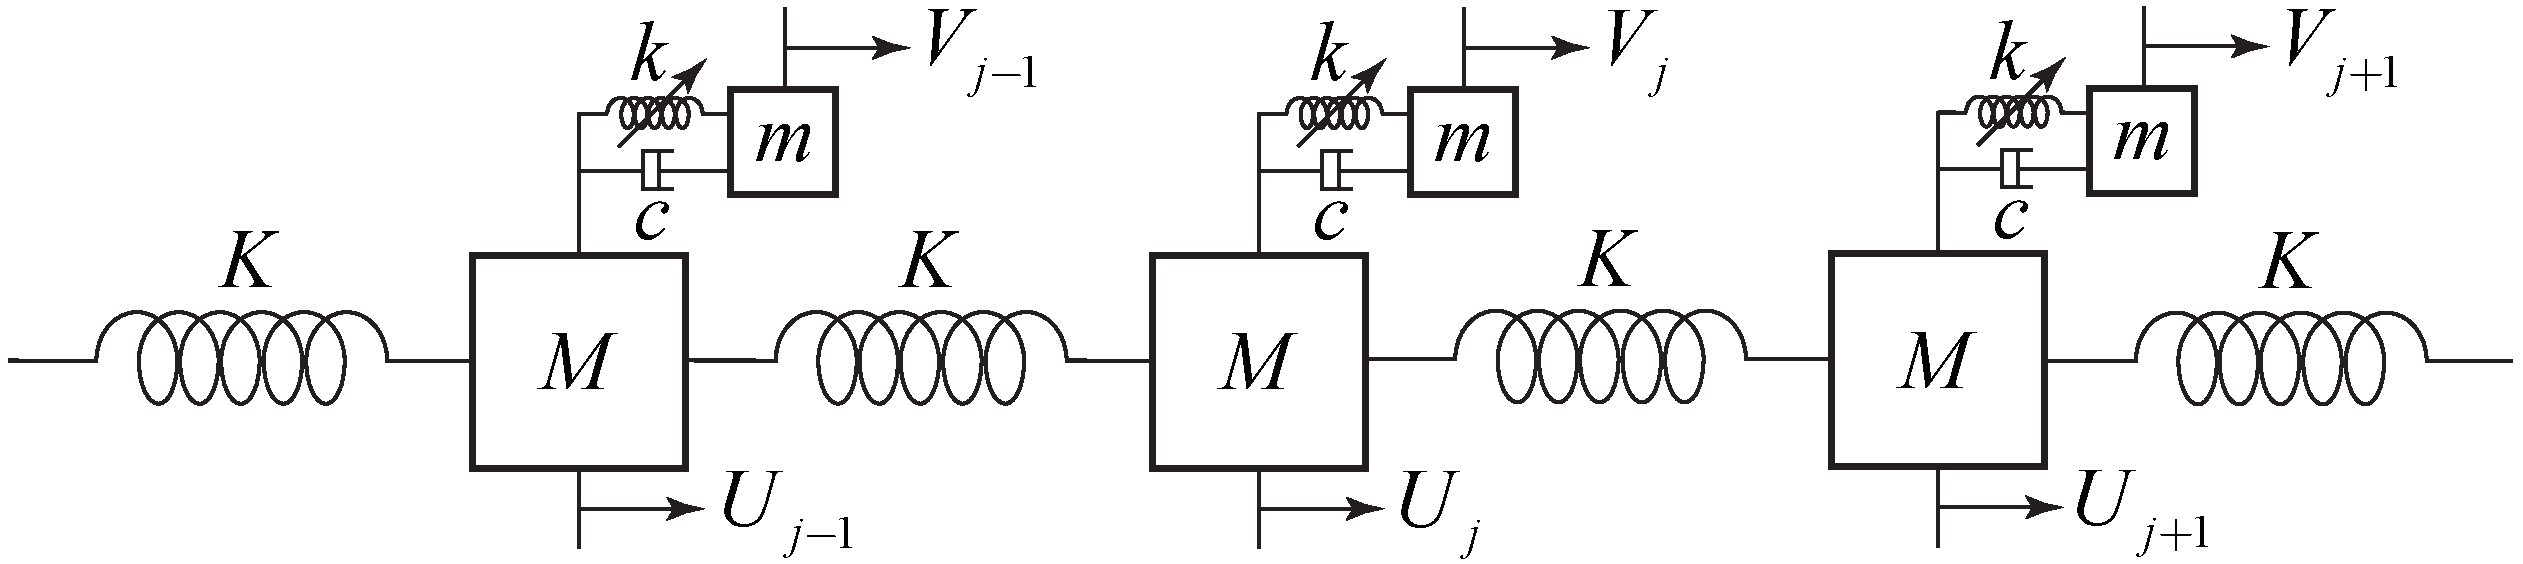
\includegraphics[scale=0.42]{slike/teorija/MM_veriga.png}
            \caption{enodimenzionalna metamaterialna veriga.}\label{fig:MM_veriga}
        \end{figure}
        
        Ko je število ROC neskončno, ali zadosti veliko, se tvori periodičnost verige, kjer ima vsaka celica periodične robne pogoje. Z $j$-to ROC lahko zapišemo gibalne enačbe: 
        \begin{align}
            M \ddot{U}_j+2 K U_j-K U_{j-1}-K U_{j+1}+c\left(\dot{U}_j-\dot{V}_j\right)+F_{\mathrm{ROC}}(U_j-V_j)&=0 \label{eq:gib_en_ROC_1} \\
            m \ddot{V}_j+c\left(\dot{V}_j-\dot{U}_j\right)+F_{\mathrm{ROC}}\left(V_j-U_j\right)&=0 \label{eq:gib_en_ROC_2} \,.
        \end{align}
        Za analizo pretvorimo enačbi v brezdimenzijsko obliko z vpeljavo: 
        \begin{align}
            &\tau=\omega_0 t, \quad  u_j=\frac{U_j}{L_0}, \quad v_j=\frac{V_j}{L_0}, \quad q_j=v_j-u_j, \quad \zeta=\frac{c}{2\sqrt{k \, m}} \nonumber \\ 
            &\alpha=\frac{k}{K}, \quad \beta=\frac{m}{M}, \quad \omega_0=\sqrt{\frac{K}{M}}, \quad \kappa_0=\sqrt{\frac{k}{m}}, \quad \varkappa=\sqrt{\frac{\kappa_0}{\omega_0}}=\sqrt{\frac{\alpha}{\beta}}\,.
        \end{align}
        Razen $\tau$, ki predstavlja brezdimenzijski čas, smo spremenljivke že definirali v poglavju \ref{sec:dvomasni_dušilec_nihanj}. Vpeljemo tudi brezdimenzijsko silo $f_{\mathrm{ROC}}=F_{\mathrm{ROC}}/(k_v L_0)$ iz dela \ref{sec:staticna_analiza_ROC}. Nadaljnji časovni odvodi diferencialnih enačb \eqref{eq:gib_en_ROC_1} in \eqref{eq:gib_en_ROC_2} so tako po brezdimenzijskem času:
        \begin{align}
            u_{j}''+2 u_{j} - u_{j-1} - u_{j+1} - 2 \zeta \beta \varkappa q_{j}' - \alpha f_{\mathrm{ROC}}(q_{j}) &= 0  \label{eq:gib_en_ROC_3} \,,\\
            q_{j}''+2 \zeta \varkappa q_{j}'+ \varkappa^2 f_{\mathrm{ROC}} (q_{j}) + u_{j}''&=0  \label{eq:gib_en_ROC_4} \,.
        \end{align}
        Za nadaljnjo analizo brezdimenzijsko silo $f_{\mathrm{ROC}}(q_j)$ v enačbi \eqref{eq:brezdimenzijski_f(x)} v okolici ravnovesne lege $q_j=0$ s pomočjo Taylorjeve aproksimacije razvijemo v:
        \begin{align}
            f_{\mathrm{ROC}}(q_j) = \frac{1}{2}\left(2+\mu-\frac{\mu}{\gamma}\right)  q_j + \frac{\mu }{4 \gamma^3} q_j^3 -\frac{3 \mu }{16 \gamma^5} q_j^5 + \frac{5 \mu}{32 \gamma^7} q_j^7 + ...
        \end{align}
        Z upoštevanjem enačb \eqref{eq:KNT_pogoj_1}, \eqref{eq:KNT_pogoj_2} ter aproksimacije petega reda dobimo:
        \begin{align}
            f_{\mathrm{ROC}}(q_j) \approx \frac{1}{2 \gamma^2(1-\gamma)} q_j^3-\frac{3}{8  \gamma^4 (1-\gamma)} q_j^5 \nonumber \,, \\
            f_{\mathrm{ROC}}(q_j) \approx \delta q_j^3 + \eta q_j^5\,.
        \end{align}
        
        Analitična rešitev nelinearnega sistema enačb \eqref{eq:gib_en_ROC_3} in \eqref{eq:gib_en_ROC_4} ni znana. Aproksimativno rešitev je mogoče dobiti z uporabo metode harmonskega ravnotežja \cite{huang2016harmonic}, \cite{thomsen2003vibrations}. Predpostavimo periodični odziv pomika $q_j(\tau)$ v obliki kompleksne Fouriereve vrste: 
        \begin{equation}
        \begin{aligned}
            q_{k, j}(\tau) &=\sum_k \epsilon^{(k-1) / 2} A_{k, j} \mathrm{e}^{\mathrm{i} k \Omega \tau}+\epsilon^{(k-1) / 2} \overline{A}_{k, j} \mathrm{e}^{-\mathrm{i} k \Omega \tau}, \quad k &=1, 3, 5, \ldots \,, 
        \end{aligned}
        \end{equation}
        
        kjer je $\epsilon$ brezdimenzijski parameter, ki kaže na red amplitude gibanja in $\Omega=\omega/\omega_0$ normirana lastna krožna frekvenca. Višje rede zanemarimo in za $k=1$ dobimo:
        \begin{equation}\label{eq:nastavek_qj}
            q_j(\tau)=A_j \mathrm{e}^{i\Omega \tau}+\overline{A}_j \mathrm{e}^{-i\Omega \tau} \,.
        \end{equation}
        
        Nastavek vstavimo v enačbo \eqref{eq:gib_en_ROC_4} in dvojno integriramo glede na $\tau$, kjer dobimo izraz odziva $j$-te mase, ter pri tem zanemarimo člene višjega reda $\mathcal{O}(A_j \mathrm{e}^{3 i \Omega \tau})$:
        \begin{align}\label{eq:nastavek_uj}
            u_j=&\frac{A}{\Omega^2}\left[ A_j \overline{A}_j (3\delta+10 A_j \overline{A}_j \eta)\varkappa^2 + 2 i \zeta \varkappa \Omega-\Omega^2 \right]  \mathrm{e}^{i \Omega \tau} + ...\nonumber\\
            & ... + \frac{B}{\Omega^2}\left[ A_j \overline{A}_j (3\delta+10 A_j \overline{A}_j \eta)\varkappa^2 + 2 i \zeta \varkappa \Omega-\Omega^2 \right] \mathrm{e}^{-i \Omega \tau}  + \mathcal{O}(A_j \mathrm{e}^{3 i \Omega \tau}) \,.
        \end{align}
        
        Nastavek \eqref{eq:nastavek_qj} in zgornjo enačbo \eqref{eq:nastavek_uj} vstavimo v \eqref{eq:gib_en_ROC_3} in nastavimo koeficiente pred $\mathrm{e}^{	\pm i \Omega \tau}$ na nič. Dobimo amplitudno-frekvenčni enačbi:
        \begin{align}
            A_{j-1}+A_{j+1}-&A_{j}\left(2+ A_{j} \overline{A}_{j}(3 \delta+10 A_{j} \overline{A}_{j} \eta)\left(\alpha+\varkappa ^2\right)\right) - ...\nonumber \\
            ... &-\frac{3\delta\varkappa^2}{\Omega^2}\left(A_{j-1}^2 \overline{A}_{j-1}-2 A_{j}^2 \overline{A}_{j}+A_{j+1}^2 \overline{A}_{j+1}\right) - ... \nonumber \\
            ... & - \frac{10\eta\varkappa^2}{\Omega^2}\left(A_{j-1}^3 \overline{A}_{j-1}^2-2 A_{j}^3 \overline{A}_{j}^2+A_{j+1}^3 \overline{A}_{j+1}^2\right) -     ... \nonumber\\
            ... &- \frac{2 i(A_{j-1}-2 A_{j}+A_{j+1}) \zeta \varkappa }{\Omega} -2 i A_{j}  (1+\beta) \zeta \varkappa  \Omega+A_{j} \Omega^2 = 0 \,,
        \end{align}
        \begin{align}
            \overline{A}_{j-1}+\overline{A}_{j+1}-&\overline{A}_{j}\left(2+A_{j} \overline{A}_{j}(3 \delta+10 A_{j} \overline{A}_{j} \eta)\left(\alpha+\varkappa ^2\right)\right) - ...\nonumber \\
            ... &-\frac{3\delta\varkappa^2}{\Omega^2}\left(A_{j-1} \overline{A}_{j-1}^2-2 A_{j} \overline{A}_{j}^2+A_{j+1} \overline{A}_{j+1}^2\right) - ... \nonumber \\
            ... & - \frac{10\eta\varkappa^2}{\Omega^2}\left(A_{j-1}^2 \overline{A}_{j-1}^3-2 A_{j}^2 \overline{A}_{j}^3+A_{j+1}^2 \overline{A}_{j+1}^3\right) -     ... \nonumber\\
            ... &- \frac{2 i(A_{j-1}-2 A_{j}+A_{j+1}) \zeta \varkappa }{\Omega} -2 i A_{j} (1+\beta) \zeta \varkappa  \Omega+A_{j} \Omega^2 = 0 \,.
        \end{align}
        
        V zgornje enačbe lahko vstavimo specifične vrednosti amplitud mase $j$ kot tudi sosednjih mas $j+1$ in $j-1$, dobimo sistem enačb za amplitudo odziva pritrjenega oscilatorja. Sistem je nelinearen in ima posledično lahko več rešitev. Amplitudo vala, ki potuje po MM verigi dobimo tako, da vstavimo amplitudo pritrjenega oscilatorja v enačbo \eqref{eq:nastavek_uj}.
        
        \newpage
        Val, ki potuje po MM verigi preko pomikov $u_j$ lahko določimo tudi tako, da definiramo faktor širjenja valovanja $\mu_u$, ki predstavlja valovno število $k_u$ pomnoženo z razdaljo med masami ROC-jev $L_u$. Pomika sosednjih mas, lahko definiramo kot:
        \begin{equation}
            u_{j \pm 1}= B_j \mathrm{e}^{\pm i \mu_u} \mathrm{e}^{\mathrm{i} \Omega \tau} + 
            \overline{B_j} \mathrm{e}^{\pm i \mu_u} \mathrm{e}^{-\mathrm{i} \Omega \tau}\,,
        \end{equation}
        
        pri čemer so $B_j$ in $\overline{B}_j$ koeficienti pred $\mathrm{e}^{\pm i\Omega \tau}$ enačbe \eqref{eq:nastavek_uj}. Zgornjo enačbo, kot tudi enačbo \eqref{eq:nastavek_qj} vstavimo v enačbo \eqref{eq:gib_en_ROC_3}, enačimo koeficiente pred $ \mathrm{e}^{\pm i\Omega \tau}$ z nič in rešimo za $\mu_u$, ter tako dobimo enačbo disperzijskih krivulj:
        \begin{align}\label{eq:disperzijska_krivulja}
            \cos{\mu_u}=1-\frac{\Omega}{2}
            -\frac{\Omega^2}{2} \left[ \frac{\alpha(3 \delta A_j \overline{A}_{j}  + 10 \eta A_j^2 \overline{A}_{j}^2  ) + 2 i \beta \zeta \varkappa \Omega}{\varkappa^2 (3 \delta A_j \overline{A}_{j}  + 10 \eta  A_j^2 \overline{A}_{j}^2 ) - \Omega^2 + 2 i \zeta \varkappa \Omega} \right] \,.
        \end{align}
        
        Disperzijske krivulje so grafično prikazane na sliki (\ref{fig:teoreticna_disperzijska}), kjer so prikazane realne in imaginarne komponente rešitve. Končno lahko zapišemo razmerje med $M_j$-to in $M_{j+1}$-to maso kot:
        \begin{equation}
            u_{j+1}=\mathrm{e}^{\Im{\mu}} u_j \, \mathrm{e}^{-i \Re{\mu}} \,.
        \end{equation}
        
        Do dušenja mehanskih valov v verigi pride v tako imenovani pasovni vrzeli, kjer je $\mathrm{e}^{\Im{\mu}}$ manj kot $1$. Valovi pri drugih frekvencah izven pasovne vrzeli, potujejo brez izgube energije. Dodatno velja, da je fazni zamik $\Re{\mu}$ potujočega vala odvisen od $\mu$. Znotraj pasovne vrzeli, je dušenje največje pri minimumu $\mathrm{e}^{\Im{\mu}}$, torej pri $\Omega=\varkappa$. Z drugimi besedami, je frekvenca vzbujanja enaka lastni frekvenci resonatorjev $\Omega=\kappa_0$.
        \begin{figure}[!hb]
            \centering
            \includegraphics[scale=0.50]{slike/teorija/disperzijska_teorija.png}
            \caption{enodimenzionalna metamaterialna veriga.}\label{fig:teoreticna_disperzijska}
        \end{figure}
        
        
        
    \chapter{Metoda končnih elementov}\label{sec:MKE}
    
    Ker ima realni metamaterial v resnici končno število reprezentativnih celic in ker so te za analitično reševanje preveč kompleksne, bomo njegovo dinamiko rešili z uporabo metode končnih elementov (MKE). V poglavju \ref{sec:meritev_materialnih_lastnosti} uporabimo MKE v povezavi z eksperimentalnimi meritvami tudi za določitev modula elastičnosti $E$ osnovnega materiala.
    
    MKE je iskanje rešitev kompleksnega realnega problema z uporabo poenostavljenega modela, ki sestoji iz številnih delov, imenovanih končni elementi (KE). Torej zvezno območje diskretiziramo v podobmočja, zato je MKE po naravi aproksimativna metoda in je uporabna takrat, kadar analitična rešitev ni mogoča.
    
    Neodvisno od geometrije in celo od vrste fizikalnega problema, ki ga želimo rešiti z MKE, so osnovni koraki formulacije vedno enaki. Preko njih bomo na osnovi pregleda literature \cite{rao2010theFEMinEngineering} izpeljali enačbe MKE in reševali dinamsko analizo lastnih nihanj DVA-ja. 
    
    \textbf{Korak 1:} Razdelitev fizikalnega modela v diskretne elemente (diskretizacija).\smallskip\newline
    Na tem mestu izberemo tip, število in velikost KE. Problem bomo reševali z splošnimi volumskimi heksaedričnimi KE. 
            
    \textbf{Korak 2:} Izbira aproksimacijskega modela.\smallskip\newline
    Izberemo obliko poljubne aproksimacijske funkcije, ki določa aproksimacijo primarne spremenljivke. Najpogosteje gre za polinomske funkcije.

    \textbf{Korak 3:} Izpeljava matrik končnega elementa.\smallskip\newline
    Za KE v svojem lokalnem koordinatnem sistemu (KS) diferencialno enačbo fizikalnega problema zapišemo kot integralsko variacijsko formulacijo. Uporabimo prej izbrano interpolacijsko funkcijo in dobimo značilne matrike sistema v lokalnem KS. Sledi transformacija koordinat v globalne matrike. 

    \textbf{Korak 4:} Sestavljanje matrik posameznega končnega elementa v sistemske matrike.\smallskip\newline
    Matrike posameznih elementov razširimo na vse prostostne stopnje in jih seštejemo.

    \textbf{Korak 5:} Upoštevanje začetnih pogojev ter robnih in prehodnih pogojev.

    \textbf{Korak 6:} Reševanje sistema enačb.
    
    Definirajmo sedaj gibalne enačbe končnega elementa za reševanje problema lastnih nihanj in jih kasneje aplicirajmo na oba uporabljena tipa končnih elementov. 

    \newpage
    \section{Gibalne enačbe končnega elementa}
    
        Pomike po območju končnega elementa $\vv U$, aproksimiramo preko diskretnih vrednosti pomikov vozlišč $\vv{Q}^e$ in matrike oblikovnih oziroma aproksimacijskih funkcij $[N]$: 
        \begin{equation}\label{eq:KE_polje_pomikov}
            \vec{U}(x, y, z, t)=\left\{\begin{array}{l}
            u(x, y, z, t) \\
            v(x, y, z, t) \\
            w(x, y, z, t)
            \end{array}\right\}=[N(x, y, z)] \vv{Q}^e(t)\,.
        \end{equation}
        Za KE lahko izrazimo specifične deformacije $\vv \epsilon$ in napetosti $\vv \sigma$:
        \begin{align}
            \vv{\varepsilon}&=[B] \vv{Q}^e \label{eq:KE_deformacije} \,, \\
            \vv{\sigma}&=[D] \vv{\varepsilon}=[D][B] \vv{Q}^e, \label{eq:KE_napetosti}
        \end{align}
        kjer je $[B]$ matrika odvodov oblikovnih funkcij in $[D]$ materialna matrika, v kateri se nahaja modul elastičnosti. Z odvajanjem enačbe \eqref{eq:KE_polje_pomikov} po času definiramo polje pomikov, kjer je $\dot{\vv{Q}^e}$ diskretna vrednost vozliščnih hitrosti:
        \begin{equation}
            \dot{\vv{U}}(x, y, z, t)=[N(x, y, z)] \dot{\vv{Q}^e}(t)\,.
        \end{equation}
        Gibalne enačbe izpeljemo preko Lagrangeve formulacije:
        \begin{equation}\label{eq:KE_Lagrange}
            \frac{\mathrm{d}}{\mathrm{d} t}\left\{\frac{\partial \mathcal{L}}{\partial \dot{Q}}\right\}-\left\{\frac{\partial \mathcal{L}}{\partial Q}\right\}+\left\{\frac{\partial E_d}{\partial \dot{Q}}\right\}=\{0\} \,,
        \end{equation}
        kjer je Lagrangian $\mathcal{L}$ definiran z razliko kinetične $E_k$ in potencialne $E_p$ energije. Za vsak element lahko kinetično, potencialno in disipacijsko energijo zapišemo kot $E_d$:
        \begin{align}
            E_k^e&=\frac{1}{2} \iiint_{V^e} \rho \dot{\vv U}^{\text{T}} \dot{\vv U} \mathrm{~d} V \,,\\
            E_p^e&=\frac{1}{2} \iiint_{V^e} \vv{\varepsilon}^{\text{T}} \vv{\sigma} \mathrm{d} V-\iint_{S^{e}} \vv{U}^{\text{T}} \vv{\overline{\Phi}} \mathrm{d} S -\iiint_{V^e} \vv{U}^{\text{T}} \vv{\overline{\phi}} \mathrm{d} V \,,\\
            E_d^e&=\frac{1}{2} \iiint_{V^{e}} c \vv{U}^{\text{T}} \dot{\vv{U}} \mathrm{~d} V \, . 
        \end{align}
        Pri tem je $\rho$ gostota in $c$ koeficient dušenja. $\vv{\overline{\Phi}}$ je vektor sil na zunanjih površinah in $ \vv{\overline{\phi}}$ vektor sil kot posledica volumskih obremenitev  elementa. 
        Seštejemo energije po posameznih elementih:
        \begin{align}
            E_k=\sum_{e=1}^{E} E_k^{e}&=\frac{1}{2} \vv{Q}^{\text{T}}\left[\sum_{e=1}^{E} \iiint_{V^e} \rho[N]^{\text{T}}[N] \mathrm{d} V\right] \dot{\vv{Q}} \,,\\
            E_p=\sum_{e=1}^{E} E_p^{e}&=\frac{1}{2} \vv{Q}^{\text{T}}\left[\sum_{e=1}^{E} \iiint_{V^e}[B]^{\text{T}}[D][B] \mathrm{d} V\right] \vv{Q} \nonumber \\ 
            &-\vv{Q}^{\text{T}}\left(\sum_{e=1}^{E} \iint_{S^{e}}[N]^{\text{T}} \vec{\Phi}(t) \mathrm{d} S^e+\iiint_{V^e}[N]^{\text{T}} \vv{\overline{\phi}}(t) \mathrm{d} V\right)-\vv{Q}^{\text{T}} \vv{F_c}(t) \,,\\
            E_d=\sum_{e=1}^{E} E_d^{e}&=\frac{1}{2} \vv{Q}^{\text{T}}\left[\sum_{e=1}^{E} \iiint_{V^{(e)}} c[N]^{\text{T}}[N] \mathrm{d} V\right] \dot{\vv{Q}} \,.
        \end{align}
        Pri tem so $\vv{Q}$ globalni vektor vozliščnih pomikov, $\dot{\vv{Q}}$ hitrosti in $\vv F_c$ vektor koncentriranih vozliščnih sil. Iz zgornjih izrazov lahko razberemo masno $[M^e]$, togostno $[K^e]$ in disipacijsko $[C^e]$ matriko posameznega elementa in vektor ekvivalentnih vozliščnih sil zaradi površinskih učinkov $ \vv F_S^e$ ter zaradi volumskih učinkov $ \vv F_V^e$:
        \begin{align}
            \left[M^{e}\right]&=\iiint_{V^e} \rho[N]^{\text{T}}[N] \mathrm{d} V \label{eq:M_matrika} \,, \\
            \left[K^{e}\right]&=\iiint_{V^e} [B]^{\text{T}}[D][B] \mathrm{d} V \label{eq:K_matrika} \,, \\
            \left[C^{e}\right]&=\iiint_{V^e} c[N]^{\text{T}}[N] \mathrm{d} V \,, \\
            \vv F_S^e&=\iint_{S^{e}}[N]^{\text{T}} \vv{\overline{\Phi}} \cdot \mathrm{d} S \,, \\
            \vv F_V^e&=\iint_{V^{e}}[N]^{\text{T}} \vv{\overline{\phi}} \cdot \mathrm{d} V \,.
        \end{align}
        Če lokalne matrike razširimo na vse prostostne stopnje in jih seštejemo dobimo masno $[M]$, togostno $[K]$ in disipacijsko $[C]$ matriko celotnega sistema. Seštevek vseh ekvivalentnih vozliščnih vrednosti sil po vseh elementih $F_S^e$ in $F_V^e$  in dodatni prispevek vseh koncentriranih vozliščnih vrednosti nam vrne globalni vektor vozliščnih sil $\vv F(t)$. Definicijo masne, togostne in disipacijske matrike upoštevamo pri energijskih izrazih, ki jih vstavimo v enačbo \eqref{eq:KE_Lagrange} in dobimo globalni sistem gibalnih enačb pridobljen z metodo končnih elementov, pri čemer je $\ddot{\vv{Q}}$ vektor globalnih vozliščnih pospeškov:
        \begin{equation}
            [M] \ddot{\vv{Q}}(t)+[C] \dot{\vv{Q}}(t)+[K] \vv{Q}(t)=\vv{F}(t) \,.
        \end{equation}
        V nadaljnji obravnavi lahko zanemarimo dušenje:
        \begin{equation}\label{eq:KE_final}
            [M] \ddot{\vv{Q}}(t)+ [K] \vv{Q}(t)=\vv{F}(t) \,.
        \end{equation}

    \section{Statična analiza pri velikih pomikih}

        Če želimo ovrednotiti nelinearne učinke KNT vzmeti poglavja \ref{sec:ROC_statika} z uporabo MKE, moramo razumeti, da obstajajo tri vrste nelinearnosti, ki jih moramo upoštevati. Materialne nelinearnosti so potrebne za napovedovanje plastičnih deformacij. Kontaktne nelinearnosti so potrebne za napovedovanje spremembe stanja in drsnega trenja med sestavnimi deli. Tretja možnost, geometrijska nelinearnost, vključuje spremembe geometrije, ki vodijo v povečanje togosti. Povzeto po \cite{Crisfield2000}.

        V enačbi \eqref{eq:KE_deformacije} smo specifične deformacije definirali kot linearne funkcije diskretnih vrednosti pomikov vozlišč $\vec Q^e$. Pri velikih pomikih ne moramo predpostaviti linearne odvisnosti deformacije. Postopamo tako, da je togost $[K]$ enačbe \eqref{eq:KE_final} funkcija pomika, zanemarimo pa tudi $[M]$:
        \begin{equation}
            [K(\vv Q)] \, \vv{Q}=\vv{F} \,.
        \end{equation}

        Ker je numerično reševanje nelinearnega problema kompleksno, postopamo tako, da rešujemo iterativno in ob vsakem časovnem koraku primerjamo linearno togost $[K]$ pridobljeno iz statičnega ravnovesja sil enačbe \eqref{eq:KE_final}  in posodobimo geometrijo. 

        
    \newpage
    \section{Analiza lastnih nihanj}\label{sec: AnalizaLastNihanj}
        Poljubnemu sistemu lahko v začetku opazovanja dodelimo neke začetne pogoje, nato pa mu prepustimo, da prosto niha. Po vnosu začetnih pogojev struktura ni pod vplivom nobene zunanje sile in pravimo, da je sistem v stanju proste vibracije  \cite{boltezar2010mehanska}.
        Matematični izhodišče pri iskanju lastnih frekvenc (lastnih vrednosti) in pripadajočih lastnih oblik predstavlja enačba \eqref{eq:KE_final}, pri čemer je $\vv F=0$:
        \begin{equation}\label{eq:gib_en_lastna}
            [M] \ddot{\vv{Q}}+[K] \vv{Q}=\vv 0\,.
        \end{equation}
        Gre za sistem $n$ homogenih gibalnih enačb, kjer je $n$ število prostostnih stopenj. Za nedušene in harmonične proste vibracije iščemo rešitev kot $n$ harmonskih funkcij zapisanih v vektorski notaciji kot:
        \begin{equation} \label{eq:harmonska_funkcija}
            \vv Q= \vv{\overline{Q}} \, e^{i \omega t} \,,
        \end{equation}
        kjer so iskane neznane vrednosti amplitude $\vv{\overline{Q}}$ in lastne frekvence $\omega$. Sistem ima $n$ lastnih frekvenc ter enako število lastnih oblik.
        Nastavek \eqref{eq:harmonska_funkcija} uporabimo v enačbi \eqref{eq:gib_en_lastna}:
        \begin{align}\label{eq:karakteristica_en}
            -\omega^2 [M]\ddot{\vv{Q}} \, e^{i \omega t}+[K]\vv{Q} \,e^{i \omega t}&=\vv 0 \, \textrm{ / predp. } \,e^{i \omega t} \neq 0\nonumber \,, \\
            \left(\,[K]-\omega^2[M] \, \right) \vv{\overline{Q}}&=\vv 0 \, \textrm{ / pomnožimo z }[M^{-1}]\nonumber \,, \\
            \left(\,[A\,]-\lambda \, [\,I\,] \, \right) \vv{\overline{Q}}&=\vv 0 \,,
        \end{align}
        kjer je matrika $[A\,]=[K][M^{-1}]$ imenovana dinamska matrika sistema. $\lambda=\omega^2$ je parameter, ki vodi do lastnih vrednosti sistema. Netrivialna rešitev zahteva vsaj eno neničelno amplitudo v vektorju $\vv{\overline{Q}}$, torej iščemo neničelnost determinante ali karakteristično enačbo sistema:
        \begin{equation}
            \det \left( \, [A\,]-\lambda \, [\,I\,] \, \right)=0 \,,
        \end{equation}
        Razvoj determinante pripelje do polinoma $n$-te stopnje:
        \begin{equation}
            \lambda^{n}+X_1\lambda^{n-1}+...+X_n=0\text{ ,}
        \end{equation}
        iz katerega izrazimo $n$ lastnih vrednosti sistema. Lastne vrednosti uredimo po velikosti $\lambda_i$, $i=1, ..., n$, tako da najmanjše število pomeni prva lastna vrednost in hkrati prva lastna frekvenca $f_0$:
        \begin{equation}\label{eq:lastna_frekvenca}
            f_{0,i}=\frac{\omega_{i}}{2 \pi}=\frac{\sqrt{\lambda_i}}{2 \pi} \, \textrm{; } i=1,\, ...\,,\,n \,.
        \end{equation}
        Z vstavljanjem izračunanih lastnih vrednosti $\lambda_i$ v enačbo \eqref{eq:karakteristica_en} izračunamo pripadajoče lastne vektorje $\overline{Q}_i$. Lastni vektorji ne predstavljajo dejanske amplitude, temveč medsebojno relativne vrednosti. Če te relativne vrednosti normiramo in formuliramo v vektor $\vv{\overline{Q}}$, ta predstavlja modalno obliko pripadajoče lastne frekvence. 
        V sistemu z velikim številom matrik (v resnici že pri $3 \times 3$ matriki) postane postopek iskanja lastnih vrednosti analitično težko rešljiv. Lastne vrednosti in pripadajoče lastne vektorje iščemo numerično. Numerične metoda hkrati vrnejo sezname lastnih vrednosti $\lambda$ ter seznam desnih normiranih lastnih vektorjev $\vv{\overline{Q}}$. 
        
    \newpage
    \section{Masna in togostna matrika končnih elementov}
        
        V izpeljavi dinamičnih enačb po metodi končnih elementov vidimo, da potrebujemo določiti masno in togostno matriko končnega elementa. Natančno geometrijo metamateriala popišemo z heksaedričnimi volumskimi KE. Te tvori osem vozlišč $i=1\text{-}8$, katerega vsako ima tri prostostne stopnje $u_i$, $v_i$, $w_i$. Izpeljavo izvedemo za izoparametrični KE, tako da je element v naravnem koordinatnem sistemu (KS) $r$, $s$, $t$ vedno kocka (slika \ref{fig:heksaedricni_KE}). Preko Jakobijeve matrike $[J]$ lahko izpeljavo v naravnem transformiramo v kartezijev KS. Velja, da lahko zaradi fizike ponekod problem obravnavamo poenostavljeno. Takrat lahko matrike poenostavimo na dvodimenzionalne. 
        \begin{figure}[!hb]
            \centering
            \includegraphics[scale=0.65]{slike/teorija/heksaedricni_KE.png}
            \caption{Heksaedrični KE v kartezijevem (levo) in naravnem (desno) KS \cite{rao2010theFEMinEngineering}. }\label{fig:heksaedricni_KE}
        \end{figure}
        
        Enačbi za masno matriko pridobljeno z \eqref{eq:M_matrika} in togostno matriko z \eqref{eq:K_matrika} se v primeru izoparametričnega heksaerdičnega KE glasita:
        \begin{align}
            \left[M^{e}\right]&=\int_{-1}^{1}\int_{-1}^{1}\int_{-1}^{1} 
            \rho \, ([J]^{-1}[N])^{\text{T}}([J]^{-1}[N]) \, \operatorname{det}[J] 
            \, \mathrm{d} r\, \mathrm{d} s\, \mathrm{d} t \,, \\
            \left[K^{e}\right]&=\int_{-1}^{1}\int_{-1}^{1}\int_{-1}^{1}
            ([J]^{-1}[B])^{\text{T}}[D]([J]^{-1}[B]) \, \operatorname{det}[J] 
            \, \mathrm{d} r\, \mathrm{d} s\, \mathrm{d} t \,,
        \end{align}
        
        kjer je matrika oblikovnih funkcij v naravnem KS: 
        \begin{align}
        &[N]=\left[\begin{array}{cccccc}
        N_{1} & 0 & 0 & N_{2} & \ldots & 0 \\
        0 & N_{1} & 0 & 0 & \ldots & 0 \\
        0 & 0 & N_{1} & 0 & \ldots & N_{8}
        \end{array}\right] \,, \\
        &N_{i}(r, s, t)=\frac{1}{8}\left(1+m_{i}\right)\left(1+s s_{i}\right)\left(1+t t_{i}\right) ; \quad i=1,\,2, \ldots, 8 
        \end{align}
        in matrika odvodov oblikovnih funkcij, ki je dimenzije $6$ x $24$:
        \begin{equation}
        [B]=\left[\left[B_{1}\right]\left[B_{2}\right] \ldots\left[B_{8}\right]\right] \,.
        \end{equation}
        Jakbijeva matrika je definirana kot:
        \begin{equation}
        [J]=
        \left[\begin{array}{ccc}
        \sum_{i=1}^{8}\left(\frac{\partial N_{i}}{\partial r} x_{i}\right) & \sum_{i=1}^{8}\left(\frac{\partial N_{i}}{\partial r} y_{i}\right) & \sum_{i=1}^{8}\left(\frac{\partial N_{i}}{\partial r} z_{i}\right) \\
        \sum_{i=1}^{8}\left(\frac{\partial N_{i}}{\partial s} x_{i}\right) & \sum_{i=1}^{8}\left(\frac{\partial N_{i}}{\partial s} y_{i}\right) & \sum_{i=1}^{8}\left(\frac{\partial N_{i}}{\partial s} z_{i}\right) \\
        \sum_{i=1}^{8}\left(\frac{\partial N_{i}}{\partial t} x_{i}\right) & \sum_{i=1}^{8}\left(\frac{\partial N_{i}}{\partial t} y_{i}\right) & \sum_{i=1}^{8}\left(\frac{\partial N_{i}}{\partial t} z_{i}\right)
        \end{array}\right].
        \end{equation}
        
        
       
       
       
        
    \chapter{Termoaktivne lastnosti GPLA}\label{sec:PLA}
    
        Bistvena lastnost polilaktične kisline ali PLA (\textit{Polylactic acid}) je steklasti prehod iz trdnega v tekoče pri temperaturi steklenja $T_g$. Pri sobni temperaturi je PLA trd in krhek, z višanjem temperature preide v steklasto stanje (od $0,8 \, T_g$ do $T_g$) in nato v gumielastično področje (od $T_g$ do $1,4 \, T_g$), kjer se material z višanjem temperature mehča a plastično ne deformira. Pri ponovnem ohlajevanju se material povrne v prvotno stanje. Pri segrevanju nad $1,4 \, T_g$ material preide v plastično in nato talilno področje \cite{Glass_transition_Wiki}. Mehčanje materiala z višanjem temperature se izraža kot padanje modula elastičnosti $E$ oziroma togosti materiala, ki je temeljna karakteristika pri obravnavi dinamskih sistemov. Naš cilj je ugotoviti povezavo med modulom elastičnosti in temperaturo in preko nje krmiliti togost metamateriala. Eksperimentalno to dosežemo v poglavju \ref{sec:meritev_materialnih_lastnosti}. 
    
        Sprva torej potrebujemo mehanizem preko katerega bomo material lahko segrevali. Osnovnemu PLA-ju lahko z različnimi aditivi spremenimo lastnosti. V naši aplikaciji je bistvenega pomena dodatek grafitnega prahu, ki tvori GPLA (\textit{Graphite Polylactic acid}). Električna prevodnost grafita znatno zniža specifično upornost $\varrho$ GPLA-ja.
    
        Električni tok $I$ pri napetosti $U$, ki teče skozi dušilec z uporom: 
        \begin{equation}\label{eq:upor}
            R=\varrho\,l / A \, ,
        \end{equation}
        kjer je $A$ površina preseka in $l$ dolžina dušilca. Tok povzroča segrevanje zaradi Joulove moči $P=I^2R$. Upoštevamo konvekcijo in zapišemo energijski zakon \cite{Soft-Actuators_Al-Rubaiai}:
        \begin{align}\label{eq:energijska_bilanca}
            m \, c_p \frac{dT(t)}{dt}&=I^2R-h_s \, A_s \left( T(t)-T_\infty \right) \, ,
        \end{align}
        kjer je $m=\rho A l$ masa dušilca z gostoto $\rho$, $c_p=1600 \text{ J/kgK}$  specifična toplota materiala \cite{Thermal-properties-of-samples} in $A_s$ celotna površina v kontaktu z zrakom s koeficientom toplotne prestopnosti $h_s$. $T=T(t)$ je temperatura vzorca ob času $t$ in $T_\infty$ temperatura okolice, pri čemer je $T(t=0)=T_\infty$. Rešimo diferencialno enačbo \eqref{eq:energijska_bilanca}:
        \begin{equation}\label{eq:temperatura_analiticno}
            T(t)=T_\infty + \frac{A\,U^2 \left( 1-e^{-\frac{A_s h_s}{A c_p l \rho}\cdot t} \right)}{A_s h l \varrho} \, .
        \end{equation}
        Pokazali smo, da lahko z električnim tokom GPLA segrejemo. Z zgornjo enačbo analitično aproksimiramo potrebno električno napetost $U=\Delta V$, da v času $t$ dosežemo potrebno temperaturo. Kasneje v eksperimentalnem delu povežemo temperaturo z modulom elastičnosti, kar pomeni, da lahko preko električne napetosti, ki jo je dokaj enostavno nadzirati, krmilimo togost metamateriala. 
        
    \newpage
    \section{Meritev materialnih lastnosti GPLA-ja}\label{sec:meritev_materialnih_lastnosti}

        Preden se lotimo izdelave in analize metamateriala, moramo raziskati materialne lastnosti, ki so potrebne za njegovo dimenzioniranje in krmiljenje temperature z enačbo \eqref{eq:temperatura_analiticno}. Na podlagi meritev in analize vzorcev določimo gostoto $\rho$, specifično električno upornost $\varrho$ in modul elastičnosti $E$ GPLA-ja v odvisnosti od temperature. Eksperimente smo opravili v sklopu \cite{Bizjan_2021}.
        
        Materialne lastnosti FFF (\textit{Fused filament fabrication}) 3D tiskanih struktur so močno odvisne od parametrov izdelave. Vzorce (slika \ref{fig:vzorci}) smo modelirali v \textit{SolidWorks} CAD programu. Tiskamo z debelino sloja $0,2 \text{ mm}$ v smeri vzporedno dolžini ($0^\text{o}$) ali v smeri pravokotno na dolžino nosilcev ($90^\text{o}$) s $100\%$ polnitvijo. Dimenzije $a = 10\text{ mm}$, $b=5\text{ mm}$, $h=2\text{ mm}$ in $t=8\text{ mm}$ so konstantne, variiramo le dolžino $l$, ki je prvič $30 \text{ mm}$ in drugič $60\text{ mm}$. S kombinacijo smeri tiska in dolžin analiziramo štiri vzorce. Uporabimo filament proizvajalca \textit{ProtoPlant} na FFF 3D printerju \textit{Ultimaker 3}.
        \begin{figure}[!hb]
            \centering
            \includegraphics[width=0.70\textwidth]{slike/metodologija/vzorci.eps}
            \caption{Geometrija vzorcev za določanje materialnih lastnosti \cite{Bizjan_2021}.}\label{fig:vzorci}
        \end{figure}

            Gostota GPLA plastike $\rho=m/V$ je bila določena na podlagi pomerjene mase $m$ in na podlagi dimenzij vzorcev izračunanega volumna $V$. Za maso je bila uporabljena tehtnica EMB 200-3 proizvajalca KERN.
            
            Volumen prvega modela znaša $V_1=34708 \text{ mm}^3$ in masa $m_1=39,53 \text{ g}$. Za drugi model je volumen $V_2=35586 \text{ mm}^3$ in masa $m_2=36,33 \text{ g}$. Gostota prvega je tako $\rho_1=1107 \text{ kg/m}^3$ in drugega $\rho_2=1105 \text{ kg/m}^3$. Povprečna gostota vseh GPLA vzorcev pri $26^{\,\circ}$C je $\rho_{GPLA}=1106 \text{ kg/m}^3$.

            Vzorce opremimo tako, da omogočimo prevajanje toka in meritev temperature. Na mestu kontakta jih prebarvamo s srebrno prevodno barvo in prelepimo s tanko bakreno žico. Na sredini namestimo termočlen tipa K, ki je sposoben meriti temperaturo od 0 do 100 $^o$C. Vzorec je del električnega merilnega vezja in deluje kot upor (slika \ref{fig:merilna_shema_a}). Padec napetosti $U$ merimo preko delilnika napetosti $U_{out}$. Tok $I$ lahko določimo z uporabo upora znane in dovolj majhne vrednosti, na katerem izmerimo napetost $U_{shunt}$. Meritev na delilniku in \textit{shuntu} pretvorimo v napetost in tok na vzorcu prek izrazov:
            \begin{align}
                U &= \frac{U_{out}}{0,09007}-U_{shunt} \,, \\
                I&=\frac{U_{shunt}}{1,1 \, \Omega} \, .
            \end{align}
            
            Temperaturo merimo na merilni kartici NI 9211, tok in napetost pa na NI 9215. Priključeni sta na računalnik, na katerem meritve analiziramo s programom \textit{LabView}. Specifično električno upornost $\varrho$ določimo z Ohmovim zakonom $R=U /I$ in enačbo \eqref{eq:upor} ter jo prikažemo v spodnjem grafu \ref{fig:spec_el_upornost}. Vidimo, da s temperaturo upornost narašča.
            \begin{figure}[!htb]
                \centering
                \begin{subfigure}{.489\textwidth}
                    \centering
                    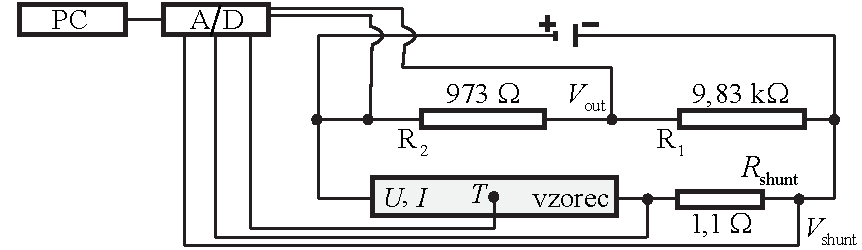
\includegraphics[width=\linewidth]{Magisterski praktikum/slike/metodologija/vezje.pdf}
                    \caption{}
                    \label{fig:merilna_shema_a}
                \end{subfigure}%
                \begin{subfigure}{.489\textwidth}
                    \centering
                    \includegraphics[trim={0.5cm 0cm 2.5cm 2cm}, clip, width=\linewidth]{Magisterski praktikum/slike/metodologija/specifična_upornost.pdf}
                    \caption{}
                    \label{fig:spec_el_upornost}
                \end{subfigure}%
                \caption{(a) Shema vezja meritve in (b) specifična upornost $\varrho$ GPLA materiala \cite{Bizjan_2021}.}
                \label{fig:merilna_shema}
            \end{figure}
            Določimo modul elastičnosti GPLA-ja ter njegovo odvisnost od temperature. Predstavimo metodo določanja modula elastičnosti materiala prek identifikacije lastne frekvence in geometrije strukture \cite{Pintelon_2003}, \cite{Kosir_2021}, ki jo analiziramo z MKE.
            Predpostavimo Hookov zakon, oziroma z drugimi besedami linearno teorijo elastičnosti, in frekvenčno neodvisnost materiala. Obravnavano geometrijo strukture rešujemo z analizo lastnih frekvenc po MKE. Izhajamo iz enačbe \ref{eq:karakteristica_en}, kjer matrike $[A\,]=[K][M^{-1}]$ vsebujejo modul elastičnosti $E$, Poissonov količnik $\nu$ in gostoto $\rho$:
            \begin{align}
                [K]&=E \, [K_0] \,,\\
                [M]&=\rho \, [M_0]\,.
            \end{align}
            $[K_0]$ predstavlja togostno matriko neodvisno od modula elastičnosti $E$ in $[M_0]$ masno matriko neodvisno od gostote $\rho$. $[K_0]$ ni povsem odvisna le od geometrije strukture, saj je še vedno odvisna od Poissonovega količnika $\nu$. Vendar če se omejimo na strukture, ki jih lahko obravnavamo kot Euler-Bernoullijev nosilec \cite{rao2007ContinuousSystems}, je $\nu$ zanemarljiv in $[K_0]$ materialno neodvisna matrika. Sistem enačb \eqref{eq:karakteristica_en}, kjer je $\lambda=\omega^2$:
            \begin{align}
                \left(\,[A\,] - \omega^2 \, [\,I\,] \, \right) \vv{\overline{Q}}&=\vv 0 \nonumber \,,\\
                \left(\,[K][M^{-1}] - \omega^2 \, [\,I\,] \, \right) \vv{\overline{Q}}&=\vv 0 \nonumber \,,\\
                \left(\,[K] - \omega^2 \, [M] \, \, \right) \vv{\overline{Q}}&=\vv 0 \nonumber \,,\\
                \left(\,E \, [K_0]-\omega^2 \rho \, [M_0] \, \right) \vv{\overline{Q}}&=\vv 0 \nonumber \,,\\
                \left( \, [K_0]-\omega^2 \frac{\rho}{E} \, [\,I\,] \, \right) \vv{\overline{Q}}&=\vv 0 \,,\nonumber
            \end{align}
            preoblikujemo v nov problem lastnih vrednosti z $\lambda=\omega^2 \rho / E$:
            \begin{align}
                \left( \, [K_0]- \lambda \, [\,I\,] \, \right) \vv{\overline{Q}}&=\vv 0 \,.
            \end{align}
            
            Materialno neodvisni lastni problem uporabimo za izračun $i$-te lastne vrednosti po MKE, ki jo povežemo z eksperimentalno izmerjeno $i$-to lastno frekvenco $f_{0,i}$, kot je definirana v enačbi \eqref{eq:lastna_frekvenca}.
            Tako je:
            \begin{align}\label{eq:karakteristica_en_modul}
                \lambda_i = 4 \pi^2 \frac{\rho}{E} f_{oi}^2 \,.
            \end{align}
            Za določanje efektivnega modula elastičnosti $E$ v nadaljevanju potrebujemo gostoto $\rho$, pomerjeno prvo lastno frekvenco $f_{0,1}$ ter po MKE izračunano prvo lastno vrednost $\lambda_1$. Na podlagi enačbe \eqref{eq:karakteristica_en_modul} lahko določimo modul elastičnosti $E$ kot:
            \begin{equation}\label{eq:modul}
                E=4 \pi^{2} \, \frac{\rho \, f_{0,1}^{2}}{\lambda_{1}} \, .
            \end{equation}
            V naslednjem koraku vzorce na mestu izoliranih (belih PLA) površin s sekundnim lepilom pritrdimo na ploščo stresalnika LDS V555 (slika \ref{fig:merilna_shema_2}). Nanjo smo namestili referenčni pospeškomer proizvajalca PCB Piezotronics, ki je povezan na tretjo merilno kartico NI 9234, na kateri je tudi laserski merilnik hitrosti Polytec PDV 100 (slika \ref{fig:merilna_shema_1}). Sedaj izvedemo modalno analizo testiranih vzorcev z MKE v programu \textit{ANSYS Mechanical} \cite{thompson2017ansys}. Poissonov količnik je privzet iz literature in znaša $\nu = 0,39$ \cite{Ferreira_2017}. Za vsak vzorec določimo matriki $[K_0]$, $[M_0]$ ter rešimo problem lastnega nihanja po enačbi \eqref{eq:karakteristica_en_modul} in izračunamo prvo lastno vrednost $\lambda_1$ (slika \ref{fig:MKE_vzorca}).
            \begin{figure}[!htb]
            \centering
            \tabskip=0pt
            \valign{#\cr
              \hbox{%
                \begin{subfigure}[b]{.45\textwidth}
                \centering
                \includegraphics[height=11cm, width=\textwidth]{Magisterski praktikum/slike/metodologija/merino_mesto_1.png}
                \caption{}
                \label{fig:merilna_shema_1}
                \end{subfigure}%
              }\cr
              \noalign{\hfill}
              \hbox{%
                \begin{subfigure}{.45\textwidth}
                \centering
                \includegraphics[height=5.0cm, width=\textwidth]{Magisterski praktikum/slike/metodologija/merino_mesto_2.png}
                \caption{}
                \label{fig:merilna_shema_2}
                \end{subfigure}%
              }\vfill
              \hbox{%
                \begin{subfigure}{.45\textwidth}
                \centering
                \includegraphics[height=4.5cm,width=\textwidth]{Magisterski praktikum/slike/metodologija/MKE_E_modul.png}
                \caption{}
                \label{fig:MKE_vzorca}
                \end{subfigure}%
              }\cr
            }
            \caption{Prikaz (a) eksperimenta za meritev modula elastičnosti (b) GPLA vzorca in (c) njegovega MKE modela za analizo lastnih vrednosti.}
            \end{figure}
            
            
            \newpage
            
            Vzorce smo vzbujali z belim šumom s konstantno amplitudo pospeška na frekvenčnem razponu od 40 do 1000 Hz. S pomerjenimi signali pospeška in hitrosti smo določili amplitudni del frekvenčne prenosne funkcije FPF vsakega vzorca pri različnih temperaturah in prvo lastno frekvenco $f_{0,1}$ (slika \ref{fig:merilna_shema_b}).  
            
            Z uporabo enačbe \eqref{eq:modul} določimo ekvivalentni modul elastičnosti GPLA materiala $E=E(T)$ in ga predstavimo v spodnjem grafu \ref{fig:modul_elastičnosti} ter določimo temperaturo steklenja $T_g=45 ^\text{ o}$C v primeru printanja pri orientaciji $0^\text{o}$. Pri tej temperaturi postane struktura stalno deformirana zaradi pričetka taljenja in se z ohlajanjem ne povrne v prvotno stanje. 
            
            Modul elastičnosti $E_{GPLA}(22^\text{ o}\text{C})=2400\text{ MPa}$ in $E_{GPLA}(42^\text{ o}\text{C})=2000\text{ MPa}$ pri orientaciji $0^\text{o}$ in  $E_{GPLA}(22^\text{ o}\text{C})=2100\text{ MPa}$ in $E_{GPLA}(35^\text{ o}\text{C})=1900\text{ MPa}$ pri orientaciji $90^\text{o}$. V nadaljevanju bomo metamaterial modelriali z uporabo kota printanja $0^\text{o}$.
            
            Tako smo določili gostoto $\rho$ in modul elastičnosti $E$, ki sta potrebni za modeliranje metamateriala, kar je naslednji korak raziskave.
            
            \begin{figure}[!htb]
                \centering
                \begin{subfigure}{.70\textwidth}
                    \centering
                    \includegraphics[width=\linewidth]{Magisterski praktikum/slike/metodologija/FRF.pdf}
                    \caption{}
                    \label{fig:merilna_shema_b}
                \end{subfigure}
                \begin{subfigure}{.70\textwidth}
                    \centering
                    \includegraphics[trim={0.0cm 0cm 2.5cm 2cm}, clip, width=\linewidth]{Magisterski praktikum/slike/metodologija/modul_elastičnosti.pdf}
                    \caption{}
                    \label{fig:modul_elastičnosti}
                \end{subfigure}
                \caption{(a) Shema vezja meritve, (b) FPF vzorca $l=60$ in $0^\circ$, (c) specifična upornost $\varrho$ in (d) modul elastičnosti $E$ GPLA pri različnih temperaturah \cite{Bizjan_2021}.}
            \end{figure}
        

    % !TeX spellcheck = sl_SI

\chapter{Zasnova metamateriala}\label{sec:Zasnova_metamateriala}

    Z definiranimi pogoji dimenzioniranja v poglavju \ref{sec:ROC_statika} in z znanimi materialnimi lastnostmi modula elastičnosti $E$ in gostote $\rho$ pridobljenimi v poglavju \ref{sec:PLA}, lahko zasnujemo in z MKE (poglavje \ref{sec:MKE}) ovrednotimo dejanski primer reprezentativne osnovne celice (ROC), ki izkazuje kvazi ničelno togost (KNT). Nato znano ROC vpeljemo v poglavje \ref{sec:dinamika_metamaterialnega_vibroizolatorja} in jo tvorimo v metamaterialno (MM) verigo, ki izkazuje lastnost pasovno zavrnitvenega filtra (PZF). Analitično verigo neskončnih členov aproksimiramo z zaporedjem desetih ROC-jev in dinamični sistem rešimo numerično. 

    \section{Zasnova in numerično vrednotenje ROC}

        Uporabimo končno enačbo (\ref{eq:kp}) pozitivne togosti poglavja \ref{sec:Izpeljava_elementa_s_pozitivno_togostjo} in enačbe (\ref{eq:kn}) negativnih togosti ter ob združitvenih pogojih (\ref{eq:k1k2k3}) za KNT dobimo dimenzijske enačbe ROC. Upoštevamo eksperimentalno pridobljen $E$ pri sobni temperaturi. Odločimo se za pravokotni prerez ROC-ja, kar vodi v vztrajnostni moment ploskve: 
        \begin{equation}
            I_1=\frac{b\, t_1^3}{l_1} \, , \,\,\,\,\,\,\,\,\,\,\,\,\,\,\,\, I_2=\frac{b\, t_2^3}{l_2} \,.
        \end{equation}
        Tako dobimo dimenzije ROC na sliki \ref{fig:ROC_dimenzija}.
        \begin{figure}[!hb]
            \centering
            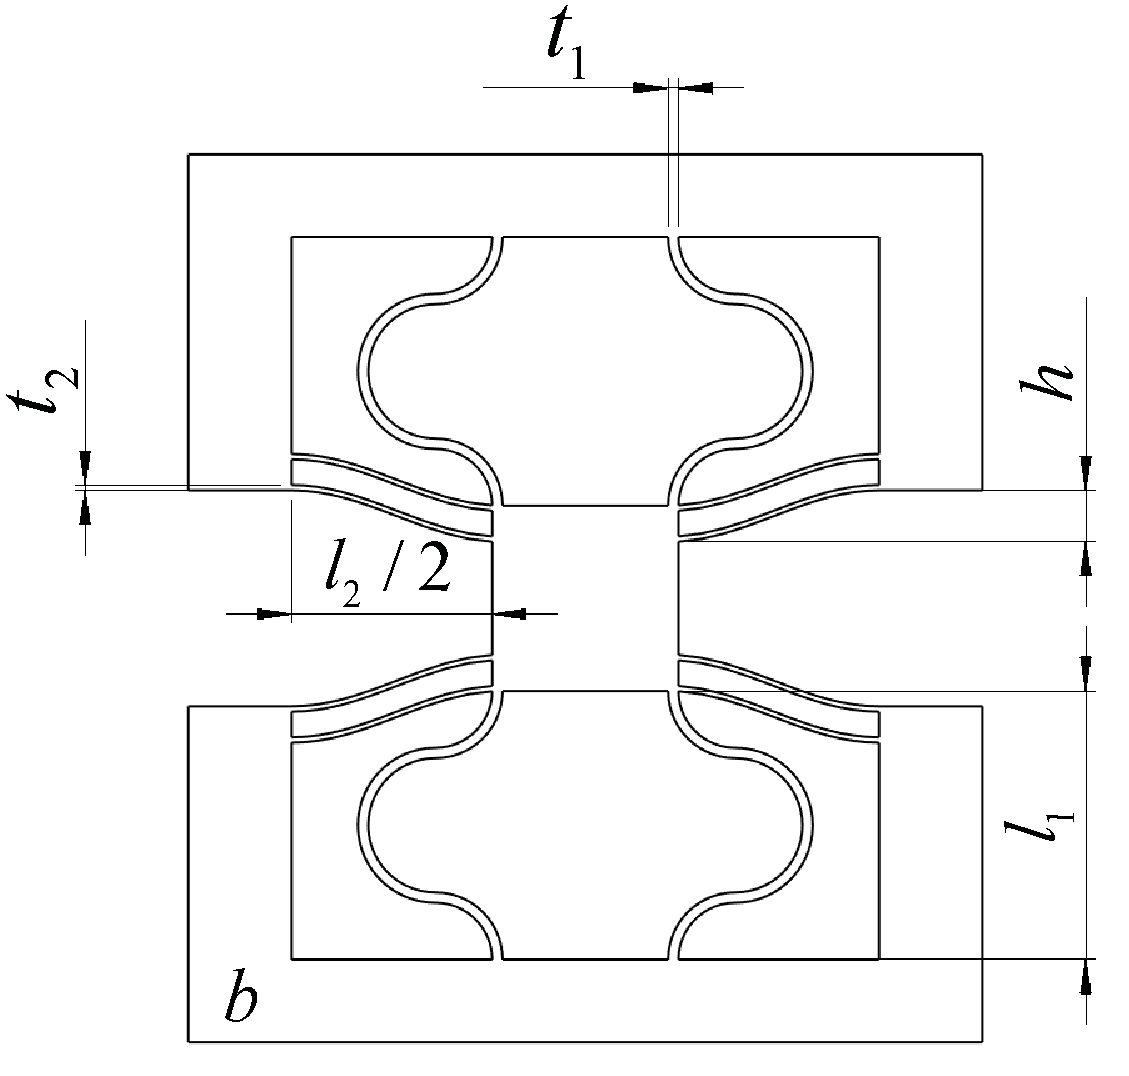
\includegraphics[width=0.51\textwidth]{Magisterski praktikum/slike/metodologija/ROC_dimenzije.png}
            \caption{Skica ROC-ja z vsemi dimenzijami.}\label{fig:ROC_dimenzija}
        \end{figure}
        
        
        
        
        Vredno omembe je povečan osrednji del za zagotovitev dovolj prostora za deformacijo in hkrati večjo resonančno maso $m$. Pomembno je tudi izpostaviti, da smo omejeni na minimalno dimenzijo šobe 3D tiskalnika, kar znaša $0,4$ mm. Torej so vse končne dimenzije faktor tega števila. 

        Za MKE analizo smo uporabili ANSYS \textit{Mechanical}. Za izvajanje statične nelinearne analize uporabimo paket, ki je namenjen analizi mehanskih struktur (slika \ref{fig:MKE_statika}). Za uporabljenim paketom stoji Ansysov skriptni jezik APDL (\textit{ang. Ansys Parametric Design Language}). Jezik nudi parameterizacijo, izvajanje logičnih funkcij in drugih kompleksnih matematičnih operacij, kar vodi v efektivni komercialni program za reševanje po MKE \cite{thompson2017ansys}. 
        
        Predpostavili smo lupino in pomrežili z 4902 elementi preko 5720 vozlišč z tipom elementa SHELL181. Vpeljali smo tudi materialni model GPLA-ja glede na meritve. 
        
        \begin{figure}[!hb]
            \centering
            \includegraphics[trim={0.0cm 0.0cm 0.0cm -2.0cm}, clip, width=0.8\textwidth]{Magisterski praktikum/slike/metodologija/MKE_statika.png}
            \caption{(a) Pomrežen model ROC-ja, (b) njegova deformirana lega z prikazano deformacijo in (c) ANSYS \textit{Workbench} shema simulacije.}\label{fig:MKE_statika}
        \end{figure}

        \newpage
        Dimenzionirano osnovno celico lahko vrednotimo z grafom sile-pomika $F$-$X$ na \ref{fig:sile_ROC} in pri tem uporabimo analitične enačbe dimenzionirana omenjene v uvodu tega poglavja, zvezno definicijo sile ROC $F_{\text{ROC}}(X)$ v enačbi \ref{eq:F-ROC} in MKE model zgoraj. 
        
        \begin{figure}[!hb]
            \centering
            \includegraphics[trim={2.0cm -1.0cm 2.0cm -2.0cm}, clip, width=1\textwidth]{Magisterski praktikum/slike/metodologija/sile_ROC.pdf}
            \caption{Analitične in numerične primerjave poteka $F$-$X$ ROC-ja.}\label{fig:sile_ROC}
        \end{figure}

        Vidimo lahko, da je analitična sila po Taylorjevi vrsti $F_{ROC}(X)$ približek diskrezno izpeljane sile zaradi togosti $k_1$, $k_2$ in $k_3$. 
        Numerični potek sile $F_{MKE}(X)$ po MKE modelu je prav tako blizu analitično določeni sili. 

        V naslednjem koraku lahko z določenimi lastnostmi togosti zasnujemo metamaterialno (MM) verigo in ovrednotimo njeno dinamiko.

    \newpage
    \section{Zasnova in numerično vrednotenje MM verige}\label{sec:zasnova_MM_verige}
        
        V naslednjem koraku grafično prikažemo enačbo disperzijske krivulje (\ref{eq:disperzijska_krivulja}) za konkretni primer metamateriala $n$-tih ROC-jev zasnovanih v prejšnjem poglavju. Preko znane geometrije in znane gostote $\rho_{GPLA}$ lahko določimo maso ROC-ja $M=1,766\text{ g}$ in maso resonatorja $m=0,145\text{ g}$. Tako lahko določimo vse brezdimenzijske vrednosti na podlagi poglavja \ref{sec:dinamika_metamaterialnega_vibroizolatorja}. 
        Določimo amplitudi $A=7$ in $B=0,007$, ter brezdimenzijsko maso $\beta = m/M = 0,082$. V grafu \ref{fig:FRF_disperzijska} prikažemo disperzijske krivulje za različne vrednosti brezdimenzijske togosti $\alpha$ in dušenja $\zeta$. Tam kjer je $\Im(\mu_u)<1$ je prenosnost vibracij zmanjšana in je prisotna pasovna vrzel. Vidimo, da je pasovna vrzel za nizko togost $k$ pri zelo nizkih frekvencah.
        \begin{figure}[!hb]
            \centering
            \includegraphics[trim={0.0cm 0.0cm 0.0cm 3.0cm}, clip, width=0.8\textwidth]{Magisterski praktikum/slike/metodologija/FRF_disperzijska.pdf}
            \caption{Disperzijska krivulja $\mu(f)$.}\label{fig:FRF_disperzijska}
        \end{figure} 
        
        \newpage
        Iz zasnovane ROC tvorimo enodimenzionalno verigo $n=10$ ROC-jev oziroma naš metamaterial (MM), ki je viden na sliki \ref{fig:MM_veriga_2}. Prva vzmet s togostjo $K=2 k_p$ je fiksno pritrjena na podlago, zadnja vzmet in tako tudi zadnja masa $M$ je prosta. Prvi ROC v verigi je harmonično vzbujen pri različnih frekvencah $f$. 
        
        Izpeljemo gibalno enačbo sistema: 
        \begin{equation}\label{eq:gibalna_enacba_MM}
            [M] \ddot{\vv{X}}(t)+[C] \dot{\vv{X}}(t)+[K] \vv{X}(t)=\vv{F}(t) \, ,
        \end{equation}
        kjer je $\vv X=\left[\begin{array}{lllllll}U_1 & Q_1 & U_2 & Q_2 & \cdots & U_n & Q_n\end{array}\right]^T$ vektor pomikov $U_j$ primarnih mas in relativnih pomikov $Q_j$ med primarno in resonančno maso za $j=1, ..., n$. Masne $[M]$, dušilne $[C]$ in togostne $[K]$ matrike so podane kot: 
        \begin{equation}
            [M]=\left[\begin{array}{ccccccc}
            M & 0 & 0 & 0 & \cdots & 0 & 0 \\
            m & m & 0 & 0 & \cdots & 0 & 0 \\
            0 & 0 & M & 0 & \cdots & 0 & 0 \\
            0 & 0 & m & m & \cdots & 0 & 0 \\
            \vdots & \vdots & \vdots & \vdots & \ddots & \vdots & \vdots \\
            0 & 0 & 0 & 0 & \cdots & M & 0 \\
            0 & 0 & 0 & 0 & \cdots & m & m
            \end{array}\right]\,,
        \end{equation}
        \begin{equation}
            [C]=\left[\begin{array}{ccccccc}
            0 & -c & 0 & 0 & \cdots & 0 & 0 \\
            0 & c & 0 & 0 & \cdots & 0 & 0 \\
            0 & 0 & 0 & -c & \cdots & 0 & 0 \\
            0 & 0 & 0 & c & \cdots & 0 & 0 \\
            \vdots & \vdots & \vdots & \vdots & \ddots & \vdots & \vdots \\
            0 & 0 & 0 & 0 & \cdots & 0 & -c \\
            0 & 0 & 0 & 0 & \cdots & 0 & c
            \end{array}\right]\,,
        \end{equation}
        \begin{equation}
            [K(Q_j)]=\left[\begin{array}{cccccccccccc}
            2 K & -k & -K & 0 & 0 & \cdots & 0 & 0 & 0 & 0 & 0 & 0 \\
            0 & k & 0 & 0 & 0 & \cdots & 0 & 0 & 0 & 0 & 0 & 0 \\
            -K & 0 & 2 K & -k & -K & \cdots & 0 & 0 & 0 & 0 & 0 & 0 \\
            0 & 0 & 0 & k & 0 & \cdots & 0 & 0 & 0 & 0 & 0 & 0 \\
            \vdots & \vdots & \vdots & \vdots & \vdots & \ddots & \vdots & \vdots & \vdots & \vdots & \vdots & \vdots \\
            0 & 0 & 0 & 0 & 0 & \cdots & -K & 0 & 2 K & -k & -K & 0 \\
            0 & 0 & 0 & 0 & 0 & \cdots & 0 & 0 & 0 & k & 0 & 0 \\
            0 & 0 & 0 & 0 & 0 & \cdots & 0 & 0 & -K & 0 & K & -k \\
            0 & 0 & 0 & 0 & 0 & \cdots & 0 & 0 & 0 & 0 & 0 & k
            \end{array}\right]
        \end{equation}

        in je $k=F_{\text{ROC}}'(Q_j)$ nelinearna togost. 
        
        Vektor sile je podan kot $\vv{F}=\left[\begin{array}{llll}f \sin (2\pi f t) & 0 & \cdots & 0\end{array}\right]^T$.

        \newpage
        \begin{figure}[!hb]
            \centering
            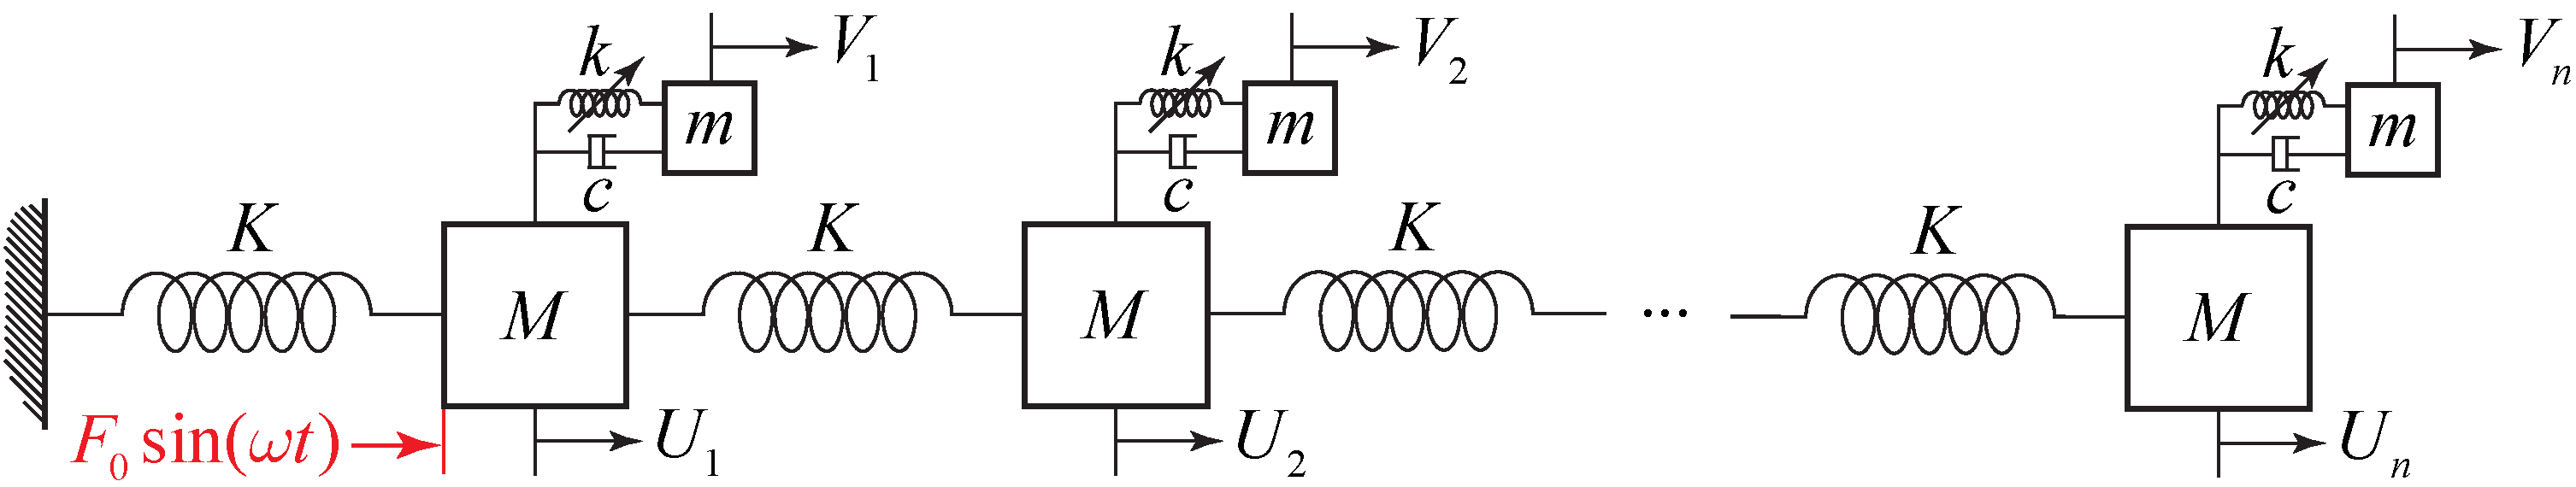
\includegraphics[scale=0.59]{slike/metodologija/MM_veriga_2.png}
            \caption{Enodimenzionalna metamaterialna veriga z robnimi pogoji.}\label{fig:MM_veriga_2}
        \end{figure}

        na spodnji sliki \ref{fig:MM_veriga_MKE} vidimo, da je dinamska numerična analiza narejena na statično predobremenjenem MM. Predobremenitev je enaka statični masi, ki jo želimo vibroizolirati. 

        \begin{figure}[!hb]
            \centering
            \includegraphics[trim={0.0cm 0.0cm 0.0cm 0.0cm}, clip, width=1.0\textwidth]{Magisterski praktikum/slike/metodologija/ROC_MKE_veriga.png}
            \caption{MM veriga z $n=10$ pri čemer je vidna predobremenitev.}\label{fig:MM_veriga_MKE}
        \end{figure}

        Problem lahko rešimo direktno z numeričnim reševanjem diferencialne enačbe pri začetnih pogojih $\vv X = \dot{\vv{X}}=\vv 0$ z uporabo implicitne Runge-Kutta sheme. Časovno integriramo pri različnih frekvencah $f$, in v frekvenčni domeni preko Fouriereve transformacije pogledamo prenosljivost $T_{\text{R-K}}$, ki je razmerje med pomikom zadnje glavne mase $U_n$ in prve mase $U_1$. 

        Indirektno lahko homogeni del gibalne enačbe (\ref{eq:gibalna_enacba_MM}) rešimo brez integriranja z linearizacijo togosti \cite{rao2017mechanical}. Če predpostavimo, da imamo dovolj majhne pomike lahko za $k\approx 0$ določimo prenosno funkcijo $T_{\text{lin}}$ z uporabo pseudoinverza:
        \begin{align}
            -\vv{X}= \left\{ [K]+ i \, \omega [D]-\omega^2 [M] \right\}^{-1} \vv{F}\,.
        \end{align}

        V sledečem poglavju si ogledamo prenosno funkcijo $T(f)$ kot končen rezultat. 








    % !TeX spellcheck = si_SI
\newpage
\chapter{Rezultati in diskusija}\label{cha:rezultati}

    Prikažemo lahko sposobnost vibroizolacije numerične analize primera metamateriala definiranem v poglavju \ref{sec:zasnova_MM_verige}. 
    V primerjavi na grafu $\abs{T(f)}$ \ref{fig:prenosna_funkcija_MM} vidimo, da se tako direktna metoda z numerično integracijo in indirektna metoda z linearizacija dobro ujemata. Opazimo lahko obstoj pasovne vrzeli v območju med $2$ in $3$ Hz. Tam se zaradi prisotnosti zavrnitvenega pasu vibracije ne prenašajo. 
    
    \begin{figure}[!hb]
        \centering
        \includegraphics[trim={0.0cm 0.0cm 0.0cm 1.0cm}, clip, scale=0.45]{Magisterski praktikum/slike/rezultati/FRF_Abs_numerika.pdf}
        \caption{Prenosnost pomika pri različnih frekvencah.}\label{fig:prenosna_funkcija_MM}
    \end{figure}

     Iz enačbe \ref{eq:disperzijska_krivulja} vidimo, da je delovanje metamateriala odvisno predvsem od dušilnega razmerja $\zeta$, masnega razmerja $\beta$ in razmerja togosti ter predvsem nelinearne togosti $\alpha$. S slike \ref{fig:FRF_disperzijska} lahko vidimo, da se z večanjem togosti pasovna vrzel pomika proti višjim frekvencam, pri višanju dušenja pa se pasovna vrzel širi, vendar je pri tem manj učinkovita.  

     Zaradi občutljivosti modula elastičnosti $E_{GPLA}$ na temperaturo, je dejanska prenosnost funkcija temperature $T=T(f, \text{temp.})$.
    % !TeX spellcheck = si_SI
\newpage
\chapter{Zaključki}\label{cha:zakljucki}

    V magisterskem praktikumu smo obravnavali dinamiko 3D natisnjenih termoaktivnih metamaterialnih blažilcev. 

    \begin{enumerate}
        \item Predstavili smo osnovno klasifikacijo metamaterialov.
        \item Predstavili smo delovanje metamateriala kot vibroabsorberja s PZF.
        \item Analitično smo izpeljali osnovno reprezentativno celico metamateriala.
        \item Obravnavali smo dinamiko neskončne periodične verige ROC-jev.
        \item Eksperimentalno smo določili modul elastičnosti $E$ in gostoto $\rho$ GPLA-ja.
        \item Numerično (z MKE) smo ovrednotili statiko ROC in dinamiko (direktna integracija sistema diferencialnih enačb) MM verige.  
    \end{enumerate}

\textbf{Nadaljnje delo}

    V magistrski nalogi nadaljujemo z izdelavo MM verige in eksperimentalnim vrednotenjem njene sposobnosti pri blaženju vibracij. Zaradi občutljivosti modula elastičnosti $E_{GPLA}$ na temperaturo, je dejanska prenosnost funkcija temperature $T=T(f, \text{temp.})$.
    Končni cilj je izdelano MM verigo, ki je prevodna, krmiliti z Joulovim tokom in se tako prilagajati spremembam temperature okolice. 
    

    \newpage
    \bibliographystyle{IEEEtran_slo}
    \renewcommand{\thechapter}{}
    \bibliography{References}
    \newpage
    % !TeX spellcheck = sl_SI
\chapter{Priloge}\label{cha:priloga}
    
    \begin{enumerate}
        \item Časovnica dela,
        \item program dela,
        \item soglasje mentorjev,
        \item zaključno poročilo o magistrskem praktikumu.
    \end{enumerate}

\includepdf[pages=-]{dodatki/Casovnica za MAGISTRSKI PRAKTIKUM - II stopnja RRP.pdf}
    \newpage
    \thispagestyle{empty}
    \mbox{}

\end{document} 